% mm comments and significant changes noted like this.


%rnaastex.cls is the classfile used for Research Notes. It is derived
%% from aastex61.cls with a few tweaks to allow for the unique format required.
%% (10/15/17)
%% (01/08/18)
\documentclass[twocolumn]{aastex62}
%\pdfoutput=1 %for arXiv submission
\usepackage{amsmath,amstext}
\usepackage[T1]{fontenc}
\usepackage{apjfonts}
\usepackage[figure,figure*]{hypcap}
%\usepackage{deluxetable}

\renewcommand*{\sectionautorefname}{Section} %for \autoref
\renewcommand*{\subsectionautorefname}{Section} %for \autoref

% citation for method paper
\newcommand{\methodpaper}{Paper I}

% line colors
\newcommand{\fiducialstyle}{black}
\newcommand{\snionstyle}{orange}
\newcommand{\snpelwstyle}{red}
\newcommand{\snonly}{dark red}

\newcommand{\shortradstyle}{light orange}
\newcommand{\RPzerostyle}{yellow} 

\newcommand{\radstyle}{light blue}
\newcommand{\ionstyle}{blue}
\newcommand{\pelwstyle}{dark blue}

\newcommand{\sfrunits}{M$_{\odot}$~yr$^{-1}$}

\newcommand{\HI}{HI}

%comment commands:
\newcommand{\aje}[1]{\textcolor{blue}{\textbf{(AJE: #1)}}}
\newcommand{\changed}[1]{\textcolor{black}{\textbf{(AJE-update): #1}}}

%% Define new commands here
\newcommand\latex{La\TeX}

%% Tells LaTeX to search for image files in the 
%% current directory as well as in the figures/ folder.
%\graphicspath{{./}{figures}}

\begin{document}

\title{The Role of Stellar Feedback in the Chemical Evolution in a Low Mass Dwarf Galaxy}

%% Note that the corresponding author command and emails has to come
%% before everything else. Also place all the emails in the \email
%% command instead of using multiple \email calls.
\correspondingauthor{Andrew Emerick}
\email{aemerick@carnegiescience.edu}

%\author{}
%\altaffiliation{}
%\affiliation{}
%% The \author command can take an optional ORCID.
\author[0000-0003-2807-328X]{Andrew Emerick}
\altaffiliation{Carnegie Fellow in Theoretical Astrophysics}
\affiliation{Carnegie Observatories, Pasadena, CA, 91101, USA}
\affiliation{TAPIR, California Institute of Technology, Pasadena, CA, 91125, USA}
\author[0000-0003-2630-9228]{Greg L. Bryan}
\affiliation{Department of Astronomy, Columbia University, New York, NY, 10027, USA}
\affiliation{Center for Computational Astrophysics, Flatiron Institute, 162 5th Ave, New York, NY, 10010, USA}
\author[0000-0003-0064-4060]{Mordecai-Mark Mac Low}
\affiliation{Department of Astrophysics, American Museum of Natural History, New York, NY, 10024, USA}
\affiliation{Department of Astronomy, Columbia University, New York, NY, 10027, USA}
\affiliation{Center for Computational Astrophysics, Flatiron Institute, 162 5th Ave, New York, NY, 10010, USA}


\keywords{Galaxy chemical evolution -- Dwarf galaxies -- Chemical enrichment -- Hydrodynamics}


\begin{abstract}
Using a suite of high-resolution simulations, we investigate how each aspect of a multi-channel stellar feedback model drives the evolution of a low-mass, isolated dwarf galaxy. Our model for star formation and stellar feedback follows individual star particles sampled randomly from an adopted initial mass function, considering independently feedback from: massive star stellar winds, AGB winds, photoelectric heating of dust grains from stellar far-ultraviolet radiation, H$_2$ dissociation from stellar Lyman-Werner radiation, and ionization, ionization heating, and radiation pressure from stellar radiation as traced with a ray-tracing radiative transfer method. We consider the effects each of these processes have on regulating the star formation rate, global gas properties and morphologies, the multi-phase interstellar medium (ISM), and driving galactic winds. In addition to total metallicity, we follow individual metal species from distinct nucleosynthetic channels (AGB winds, massive star stellar winds, core collapse supernovae, and Type Ia supernovae) and pay particular attention to how these feedback processes regulate turbulent metal mixing in the ISM, the metal content of galactic outflows, and the stellar abundances patters in our dwarf galaxy. In summary, we find that -- for a low-metallicity, low-mass dwarf galaxy -- stellar radiation, particularly ionizing radiation and H$_2$ dissociation from LW radiation, are important sources of stellar feedback whose effects are subdominant to photoelectric heating and HI radiation pressure. However, these feedback channels are coupled non-linearly, and the inclusion / exclusion of each does have non-neglible effects on particular properties of our galaxy.
\end{abstract}

\section{Introduction}

It is clear that the complex, multi-physics story of galaxy evolution is driven significantly by stellar feedback. Feedback processes regulate the formation of stars by destroying cold, star-forming gas, providing thermal pressure support and energy to prevent gas from cooling and collapsing into star-forming regions, and by driving metal-rich outflows (see \citet{Zhang2018} for a recent review), depleting galaxies of the gas required to form more stars. In addition, stellar feedback helps to drive turbulence in the interstellar medium (ISM) of galaxies, which in turn helps to mix new metal enrichment from stellar winds and supernovae in the ISM, driving galactic chemical evolution, and regulates the phases of galaxies' multi-phase ISM. The successes of modern theoretical models of galaxy evolution (see \citet{Vogelsberger2020}) are owed in large part to advances made in modelling the complex process of stellar feedback (see \citet{SomervilleDave2015} and \citet{NaabOstriker2017} for recent reviews). It has become evident that supernovae feedback alone -- a significant source of thermal and kinetic energy and momentum feedback in galaxies -- is insufficient for fully modelling the evolution of galaxies. This has driven the push for models of multi-channel stellar feedback which may include models for stellar winds, stellar radiation, and cosmic rays in addition to supernovae (give some references) \citep[e.g.][]{FIRE2,Hopkins2020}. However, the complexities in following each of these processes has precluded the development of a fully self-consistent model for multi-channel stellar feedback capable of faithfully reproducing all galaxy properties. 
%In particular, how stellar feedback couples to the multi-phase ISM and 

In pursuing this goal, high-resolution simulations of galaxy evolution capable of resolving the effects of individual feedback processes are required. The small physical sizes, low star formation rates, and relative simplicity of low-mass dwarf galaxies offers a computationally feasible regime to explore different mechanisms of stellar feedback. Simulations of dwarf galaxies have been used extensively in recent literature for this exact purpose. These models have been used to determine the efficacy of various mechanisms for depositing the energy and momentum associated with supernova feedback \citep{Smith2018b,Hu2019}, the importance of discrete, stochastic sampling of the initial mass function (IMF) in modelling individual supernova explosions \citep[e.g.]{Revaz2016,Su2018,Applebaum2020}, the role of various forms of feedback in driving metal-rich galactic winds and dwarf galaxy self-quenching \citep[e.g.][]{MacLowFerrara1999,RecchiHensler2013,Robles-Valdez2017}, with recent focus particularly on the lowest mass dwarf galaxies \citep[e.g.][]{Bland-Hawthorn2015,Cashmore2017,Romano2019}, the role of photoelectric heating in concert with other mechanisms for stellar feedback in regulating star formation and the warm, neutral ISM in dwarf galaxies \citep{Forbes2016,Hu2015,Hu2017}, the importance of ionizing radiation and radiation pressure in driving dwarf galaxy evolution \citep[e.g.][]{WiseAbel2012, Emerick2018a, Agertz2020}, feedback from high-mass X-ray binaries \citep{Artale2015,Garratt-Smithson2019}, momentum injection from resonant Ly$\alpha$ scattering \citep{Kimm2018}, the role of cosmic rays in dwarf galaxy evolution \citep[e.g.][more]{Chen2016}, and how stellar feedback drives turbulent metal-mixing in dwarf galaxies \citep[e.g.][]{Ritter2015,Corlies2018}.

The general conclusions from these studies are that stellar feedback in low-mass dwarf galaxies is effective, driving significant, metal-rich galactic winds. While SNe are perhaps the dominant mechanism by which these winds are driven, these works demonstrate that a feedback phase before the first supernova occurs in a star formation event ($\sim$ 40~Myr) is a critical component to a complete model for stellar feedback. Stellar radiation (e.g. ionization, ionization heating, radiation pressure, photoelectric heating, and Lyman-Werner dissociation of H$_2$) and, to a lesser degree, stellar winds, are important sources of this pre-SNe feedback. Not only do these processes help regulate star formation, ISM properties, and drive outflows in their own right, but these works demonstrate that they couple non-linearly to SNe feedback, decreasing he typical densities and modifying ISM structure within which SNe explode, increasing their effectiveness. 

In spite of this progress in our understanding of the role of stellar feedback in galaxy evolution, there remains gaps in our understanding. \textbf{Motivate why we need another study (mine) of this... maybe just motivate attention to chemE here}.


%\citet{Hu2015,Hu2017} SNe, radiation, PE heating
%\citet{Hu2019} individual SN models
%\citet{Forbes2016} PE heating
%\citet{WiseAbel2012} Radiation pressure
%\citet{Su2018} discrete IMF sampling in dwarfs
%\citet{Applebaum2020} discrete IMF sampling
%\citet{Agertz2020} special focus on this. with / without RT
%\citet{Kimm2018}
% ------------------ \citet{Lahen2020} detailed Hu-feedback + clusters in DG merger but no explicit testing of feedback model
% \citet{Smith2018a} \citet{Smith2018b} high res dwarfs with different models for SN feedback, concluding that other processes are important
%-------------- \citet{Koudmani2019} AGN in dwarfs

%\citet{Garratt-Smithson2019} defs summarize 
% \citet{Romano2019}

%more massive galaxies:
%FIRE (obviously)
%\citet{Benincasa2019} (and 2016?) FUV in MW galaxy. FUV alone doesn't work, but does drive WNM and leads to "softer" feedback than SN alone while still getting right masses.

%reviews:
%winds \citet{Zhang2018}
%\citet{Vogelsberger2020} defs cite somehow

This work builds upon the simulations presented in \citet{Emerick2019} (hereafter, \methodpaper) by examining in greater detail the effects of each component of our multi-channel model for stellar feedback. Our fiducial model follows star formation using individual star particles, capturing the feedback from massive star stellar winds, AGB winds, H~I and HeI ionizing radiation followed with ray-tracing radiative transfer, HI radiation pressure, photoelectric heating from far-ultraviolet (FUV) band radiation, H$_2$ dissociation from Lyman-Werner band radiation, and core collapse and Type Ia supernovae. In \citet{Emerick2018a}, we investigate the impact stellar ionizing radiation has on regulating the star formation and driving outflows in our simulated dwarf galaxy by comparing our fiducial simulation to a run without ionizing radiation and a run with only localized (within XX~pc of a massive star) ionizing radiation feedback. Expanding this analysis significantly, in this work we utilize a suite of 15 simulations which turn on / off each of these processes and examine how each drives the evolution of a low-mass ($M_{\rm vir} \sim 10^{9}$), isolated dwarf galaxy. Complimenting previous works in this regime, we pay unique attention to the role these feedback processes have on driving the individual gas-phase and stellar abundance patterns in our simulated galaxy.

\section{Methods} 
\label{sec:methods}
We refer the reader to Paper I for a detailed description of our numerical methods, initial conditions, and feedback and chemical evolution model. We briefly summarize the key components of these methods most relevant to this work below. 

We follows the evolution of an idealized, isolated, low-mass dwarf galaxy with an initial gas mass of $M_{\rm gas} = 1.80 \times 10^6$~M$_{\odot}$ initialized as an exponential disk with radial and vertical scale heights of 250~pc and 100~pc respectively. This galaxy is embedded in a static, \cite{Burkert1995} dark matter potential with virial mass and radius $M_{\rm vir} = 2.48\times 10^{9}~M_{\odot}$ and $R_{\rm vir}~=~27.4$~kpc. This is evolved using the adaptive mesh refinement hydrodynamics code \textsc{Enzo} \citep{Enzo2014}, with a minimum/maximum spatial resolution of 921.6~pc / 1.8~pc in the simulations presented in Paper I. Due to computational constraints, we were unable to perform this study at full resolution, and instead adopt 3.6~pc as the maximum resolution. We refer the reader to the resolution studies comparing maximum resolutions of 1.8~pc, 3.6~pc, and 7.2~pc performed in Paper I and \cite{Emerick2018b}. % I may need to say more here about what exactly the resolution studies show. Mostly 1.8 / 3.6 is OK but definitely large difference moving to 7.2 pc. 
The grid is refined to maintain a mass resolution of 50~M$_{\odot}$ per cell, and to ensure that the Jeans length is resolved by at least eight cells. In addition, a three-zone radius region around any star particle that has active feedback (stellar winds or SNe) is refined to the maximum grid resolution. We use the chemistry and cooling package \textsc{Grackle} \citep{GrackleMethod} to solve a nine species non-equillibrium chemistry model that includes gas-phase and dust H$_2$ formation, a uniform UV background, and localized self-shielding. This galaxy has an initial total metal mass fraction of $5.4 \times 10^{-4}$ (or $0.03 Z_{\odot}$ taking $Z_{\odot}$ = 0.018 from \cite{Asplund2009}). We follow the evolution of 15 individual metal species, C, N, O, Na, Mg, Si, S, Ca, Mn, Fe, Ni, As, Sr, Y, and Ba, whose initial mass fractions are initialized to near-zero (10$^{-20}$). Only the total metallicity affects the physics in our simulation, not the individual metal abundances. 

\subsection{Star Formation and Stellar Feedback}
\label{sec:sf feedback}

Our simulation stochastically forms star particles in dense gas ($n > 50$~cm$^{-3}$ in the 3.6~pc resolution runs presented here) by randomly sampling a \cite{Salpeter1955} IMF and depositing individual star particles from 1~M$_{\odot}$ to 100~M$_{\odot}$. For stars above 8~M$_{\odot}$, we follow their H~{\sc i} and He~{\sc i} ionizing radiation using the adaptive ray-tracing radiative transfer method of \cite{WiseAbel2011}, and trace their radiation in the Lyman-Werner and FUV bands using an optically thin approximation. These stars eject mass and energy over their lifetimes through stellar winds, and we include mass and thermal energy injection of both core collapse and Type Ia SNe. Stars below 8~M$_{\odot}$ have no feedback during their lifetime, except mass and energy deposition of their AGB winds at the end of their life. For stellar winds and SNe, mass, energy, and metals are injected to the grid by mapping a three-cell spherical region ($r=3 \times dx = 7.2~$pc) to the grid using a cloud-in-cell interpolation scheme. To reduce the significant computational expense of following a continuous source of hot ($T > 10^6$~K), fast ($v \sim 10^{3}$~km~s$^{-1}$) moving gas, we greatly reduce all stellar wind velocities to 10~km~s$^{-1}$. Given this reduction, we cannot make any strong statements as to the role of stellar wind feedback in the evolution of low mass dwarf galaxies. 

Both HI and HeI ionizing radiation is followed using the adaptive ray-tracing radiative transfer method of \cite{WiseAbel2011} and coupled to the non-equillibrium chemistry and cooling / heating routines in \textsc{GRACKLE}. Stars in our simulation use the \textsc{OSTAR2002} \citep{Lanz2003} grid of O-type stellar models to compute the HI, HeI, FUV, and LW band fluxes as a function of stellar surface gravity and surface temperature. These latter two quantities, in addition to stellar radius, are taken as a function of mass and metallicity from the \textsc{Parsec} \citep{Bressan2012,Tang2014} grid of stellar models. For stars with stellar properties off of the \textsc{OSTAR2002} grid, we adopt the associated black body flux given the stellar surface temperature. The resulting black body fluxes were adjusted to produce a continuous curve of flux as a function of stellar mass, separately in each band. Rather than adopting fixed HI and HeI photon energies for each star, we adopt the average photon energy weighted by the associated black body curve in each band, leading to HI and HeI ionzing photon energies that span the range 13.6-22.5~eV and 25.0-32.5~eV respectively, depending on stellar surface temperature. We refer the reader to Appendix~B of Paper I which contains plots of each of these quantities. In our fiducial simulations, we include the effects of radiation pressure on \HI but ignore the absorption of ionizing radiation by dust and re-radiation in the infrared.

We assume FUV and LW band radiation are both optically thin, with local (cell-by-cell) attenuation. LW radiation causes $H_2$ dissociation, while FUV radiation leads to PE heating of dust grains. We follow the PE heating models from \cite{Wolfire2003} and assuming the dust-to-gas scaling with metallicity in \cite{Remy-Ruyer2014} which shows a significant decline in the dust content at low-metallicities ($Z < 0.1$~Z$_{\odot}$). Our photoelectric heating rate is given as
\begin{equation}
    \Gamma_{\rm PE} = (1.3 \times 10^{-24} \rm{erg s^{-1} cm^{-3}}) \epsilon n_{\rm H} G_{\rm eff} D
\end{equation}
where $\epsilon$ is an efficiency factor that in detail depends upon $G_o$, temperature, and the electron number density, but which we adopt to scale weakly with $n_{\rm H}$ (see Paper I), $D$ is the dust-to-gas ratio, and
\begin{equation}
    G_{\rm eff} = G_o \rm{exp}(-1.33\times 10^{-21} D N_{\rm H})
\end{equation}
is the locally-attenuated FUV flux. $G_o$ is the FUV flux normalized to the solar neighborhood \citep{Habing1968} and $D$ is normalized to the solar value, 6.617 $\times 10^{-3}$. This model is similar to that used in both \cite{Forbes2016} and \cite{Hu2017}, with the exception of the treatment of $\epsilon$ and $D$. However, we note that both of their galaxies were at or above the $Z > 0.1$~Z$_{\odot}$ threshold and therefore have a significantly higher (but still low) dust content. We do not account for $H^-$ photodetachment due to the ISRF, which plays an important role in producing $H_2$ in our low-metallicity, low-dust content galaxy. However, we find that this effect is likely subdominant as long as either ionization or LW radiation are followed (see Appendix E of Paper I).

\section{Simulations}
\label{sec:runs}

We present the 17 different simulations run varying feedback effects in Table~\ref{table:runs}. Each simulation turns on / off various feedback processes as shown in the table. In each case, supernovae and stellar winds are included as a pair in each simulation, though again we note that we do not fully capture the effects of stellar winds in our simulations. All runs contain the same total metal enrichment from SN, massive star stellar winds, and AGB winds. In runs without SN and stellar winds, the mass and metal ejecta from these channels are instead injected at low velocity (10 km~s$^{-1}$) with a thermal energy equal to the stellar surface temperature. All runs with ionizing radiation include radiation pressure on \HI, except when noted. We test the role of radiation pressure by varying its strength with a constant factor, turning it off in RPx0, and increasing it in RPx2, RPx5, and RPx10. The shortrad simulation is the same as the fiducial simulation, but photons are deleted once they have travelled more than 20~pc from their source. This is an attempt to approximate localized prescriptions for ionizing radiation feedback which only deposit energy / ionize gas in a localized region around a star particle. We examine the effects of stellar ionizing radiation in our high-resolution (1.8~pc) simulations in \cite{Emerick2018a}, comparing our fiducial run with a shortrad simulation and a simulation without ionizing radiation (i.e. SN+PE+LW), each at 1.8~pc resolution.

All simulations are restarted from the same output after the initial collapse phase of the galaxy and formation of the first star particles.\footnote{Due to minor updates to this version of \textsc{Enzo} and the master branch of \textsc{Grackle} since publication of \methodpaper, the 3.6~pc fiducial resolution simulation presented here was re-run in its entirety and is not the same showed in the Appendix of that work.} Therefore, each run starts with the same 38 initial stars, with total stellar mass of 100 M$_{\odot}$. Three of these stars are above the 8~M$_{\odot}$ threshold for radiation and CCSNe, the most massive of which is 11 M$_{\odot}$.

% but differs only in the assumed efficiency parameter ($\epsilon$). \cite{Forbes2016} adopts a constant $\epsilon$ (\aje{I'm not sure the exact value}) while \cite{Hu2017} uses the full temperature and electron number density ($n_e$) dependent form from \cite{Wolfire2003}. However, we do not follow the necessary carbon chemistry needed to accurately follow $n_e$ in dense, neutral regions. Instead, we adopt a weak power-law fit in $n_H$ 

\begin{deluxetable*}{c|c|c|c|c|c|c}
\label{table:runs}
\tablecaption{A list of the feedback physics included in each of our runs. In every case, metal enrichment from SNe and stellar winds are kept fixed. Runs with SNe and stellar winds turned off simply replace the proper energy injection with return equal to the stellar surface temperature. The Shortrad simulation does include full radiative transfer, but deletes photons once they have travelled 25~pc from their source. The final column lists the final run time of each simulation.}
\tablehead{
\colhead{Run Name} & \colhead{SN} & \colhead{Stellar Winds} & \colhead{Ionizing Radiation} & \colhead{PE Heating + LW Radiation} & \colhead{Radiation Pressure Factor} & \colhead{End Time (Myr)}
}
\startdata
 Fiducial  & Yes & Yes & Yes & Yes       & 1  & 750 \\
 SN+Ion+PE & Yes & Yes & Yes & PE only   & -  & 552 \\
 SN+Ion+LW & Yes & Yes & Yes & LW only   & -  & 626 \\ 
 SN+Ion    & Yes & Yes & Yes & No        & 1  & 750 \\
 SN+PE+LW  & Yes & Yes & No  & Yes       & 1  & 360 \\
 SN+PE     & Yes & Yes & No  & PE only   & - & 300 \\
 SN+LW     & Yes & Yes & No  & LW only   & - & 412 \\ 
 SN-only   & Yes & Yes & No  & No        & -   & 142 \\
 RPx0      & Yes & Yes & Yes & Yes       & 0   & 750 \\
 RPx2      & Yes & Yes & Yes & Yes       & 2   & 704 \\
 RPx5      & Yes & Yes & Yes & Yes       & 5   & 750 \\
 RPx10     & Yes & Yes & Yes & Yes       & 10  & 717 \\
 Shortrad  & Yes & Yes & Yes* & Yes      & 1  & 613 \\
 Ion+PE+LW & No & No & Yes & Yes    & 1 & 750 \\ 
 Ion       & No & No & Yes & No    & 1 & 750 \\ 
 PE+LW     & No & No & No & Yes & - & 750 \\
 NoFeed    & No & No & No & No  & - & 60 
\enddata
 
\end{deluxetable*}

\section{Results}

\subsection{Star Formation Regulation}
\label{sec:sfr}

In Figure~\ref{fig:SFR} we compare the star formation rate as a function of time for each of our runs. As discussed in \methodpaper, the SFR evolution for the higher resolution fiducial simulation exhibits an initial burst up to $1 \times 10^{-3}$~M$_{\odot}$~yr$^{-1}$ followed by a lower-average, bursty SFR ($<$SFR$> = 1.19\times 10^{-4}$~M$_{\odot}$~yr$^{-1}$) with periods of up to 50-100~Myr with no star formation. This behavior is found also in the lower resolution fiducial simulation shown here (\fiducialstyle), albeit with a lower initial peak SFR and less dramatic fluctuations in SFR.
%\footnote{Our star formation algorithm has a minimum threshold gas mass to convert into stars in a single time-step, 100~$M_{\odot}$. SFR here is plotted in 10~Myr bins, yielding an effective SFR floor of $10^{-6}$ \sfrunits in Figure~\ref{fig:SFR}.} 
The most immediately visible difference between each of the runs is the magnitude of the initial burst of star formation in the first $\sim$100~Myr. Aside from the NoFeed simulation (grey) -- which rapidly forms more stars in 50~Myr than the cumulative throughout of any of the other simulations -- the SN only run (red) forms the most stars during this time. The peak SFR for each run is ranked quite nicely depending upon the feedback physics included, with PE heating producing the least change from the SN only run, up to ionizing radiation producing the largest change. PE seems to have very little effect on the initial evolution, with LW radiation and ionizing radiation generating the most significant changes. In fact, SN+Ion+LW and the three runs with no SN but do include either LW or ionizing radiation all have very similar initial bursts of star formation. The only exception to this trend is the shortrad run and Ion+PW+LW, which both have slightly smaller initial bursts. These similarities and the irrelevance of SN feedback on this early phase are clear indications that pre-SN feedback through radiation is important for star formation regulation. %During this initial phase, these runs show that, while together PE heating and LW radiation do have an effect on the SFR in the absence of ionizing radiation, ionizing radiation dominates when all three effects are included.

\begin{figure*}
  \centering
  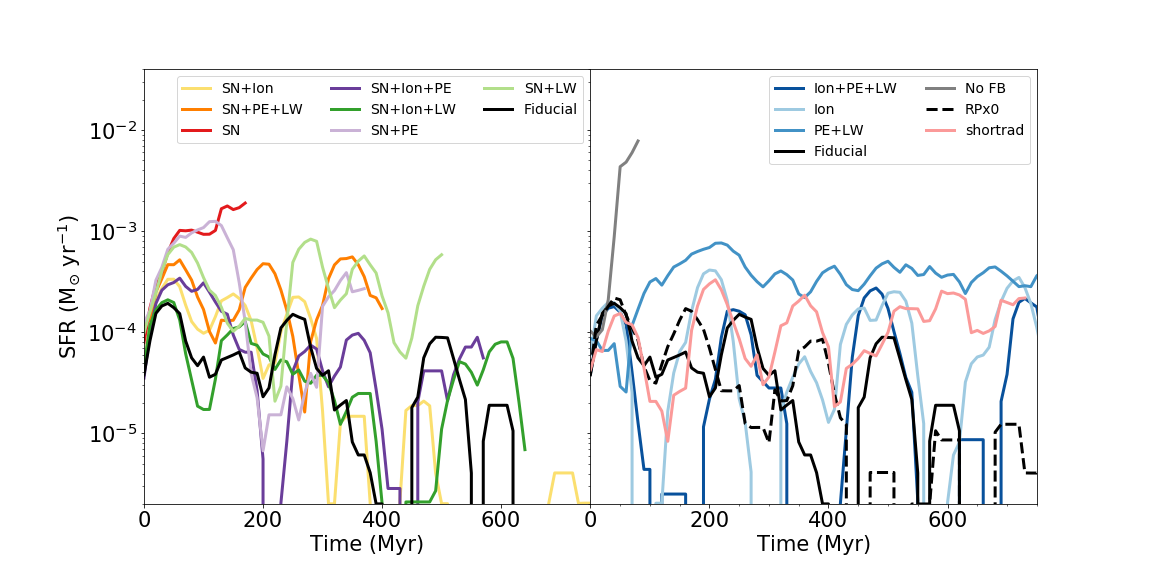
\includegraphics[width=0.98\linewidth]{figures/physics_comparison_sfr}
  \caption{The 50~Myr time-averaged SFR in each of our runs, comparing those with SN feedback (left) to those without SN (right). The fiducial simulation, which includes all physics, is plotted in both panels (\fiducialstyle) for comparison. \changed{[Smoothed in 50Myr]}}
  \label{fig:SFR}
\end{figure*}

After the first 100~Myr, the differences between runs by the inclusion of SN feedback becomes obvious. 
% AE: NOTE TO INCLUDE FOLLOWING RESULT AS A SUMMARY POINT (conclusion)
Each of the SN-included runs (left panel) show various degrees of bursty star formation for the remainder of the simulation time, with lower average star formation rate than the ionization runs. The run with only PE heating and LW radiation, PE+LW (\pelwstyle), shows the most steady SFR, indicating that this feedback channel alone is capable of producing a self-regulating SFR in this galaxy, but not the bursty star formation that is seen with the inclusion of any other feedback channel. Ionization alone (\ionstyle) and the combined radiation run (\radstyle) both show bursty star formation like the SN runs, but still have a higher average SFR and more consistent SF through the end of the simulation. The SN runs have progressively lower SFR and longer quiescent periods as each simulation proceeds.

%(\aje{Maybe show summary table of comparison values? average SFR, average retention fractions, average outflow, etc.?... maybe do this in discussion?})

\subsection{Galaxy Morphology}
\label{sec:morphology}


We show a comparison of gas morphology of our low-mass dwarf galaxy in edge-on and face-on density-weighted projections of gas number density in Figure~\ref{fig:panel_plot_1} and Figure~\ref{fig:panel_plot_2} respectively at 125~Myr for each simulation. In every simulation with SNe (top two rows and bottom left), the gas disk is puffier with a larger scale height, and with significant diffuse, outflowing gas above and below the disk. This is not true for the runs with only radiation (bottom row), which exhibit thin disks with no significant outflowing gas; however though ionizing radiation is capable of heating the disk somewhat. 

\begin{figure*}
  \centering
  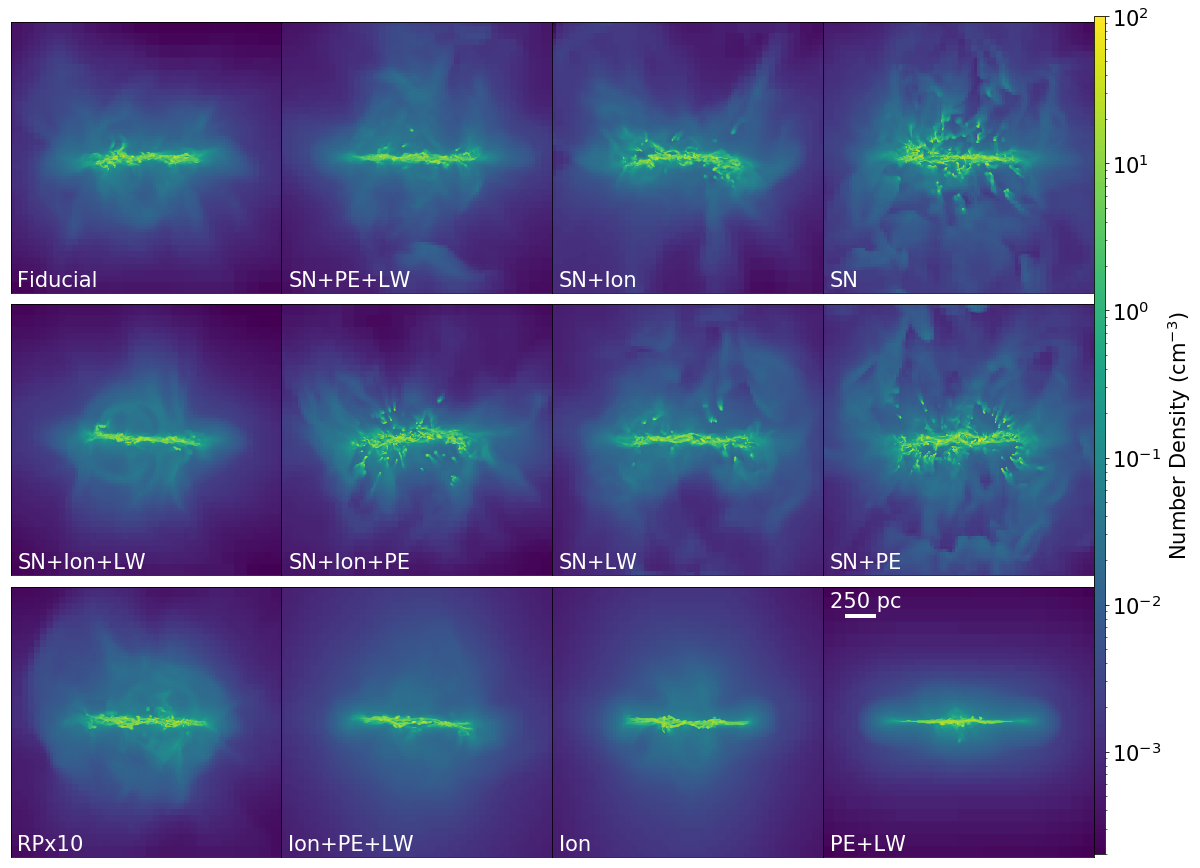
\includegraphics[width=0.95\linewidth]{figures/proj_plot_n_x_125.png}
  \caption{Edge-on projections of gas number density for each of our runs at time $t=125$~Myr.}
  \label{fig:panel_plot_1}
\end{figure*}

A subset of these runs show significant extra-planar gas structures, both in the form of diffuse shells of gas and small ($\sim$10~pc), dense clumps of gas above / below the disk (most significantly, SN, SN+Ion+PE, and SN+PE). Based upon visual analysis of the evolution of these panels, some of the diffuse shells are gas captured in an outflow / re-accretion cycle, while others are gradually pushed out due to continuing outflows. The dense clumps generally originate in the ISM and are entrained in the outflows. These clumps are still bound to the galaxy, and are ablated by the more rapidly moving diffuse gas outflows, giving rise to trailing tails of gas. In some cases these clumps are fully ablated and destroyed, while in others they persist, remain bound to the galaxy, and fall back in on an orbit with larger vertical motions than what is typical of other cold gas in the disk. These clumps do appear at some point in all simulations with either SNe or ionizing radiation, but to a much smaller extent than the obvious cases shown here. Our higher resolution fiducial simulation presented in Paper~I did show some of these features, but again not to the extreme shown here. \changed{This suggests that the presence of these clumps may be the resolution dependent, and the result of artificially strong cohesion in under resolved dense gas \citep{MacLowZahnle1994}. Confirming the physical nature of these clumps will require additional work.} H

\begin{figure*}
  \centering
  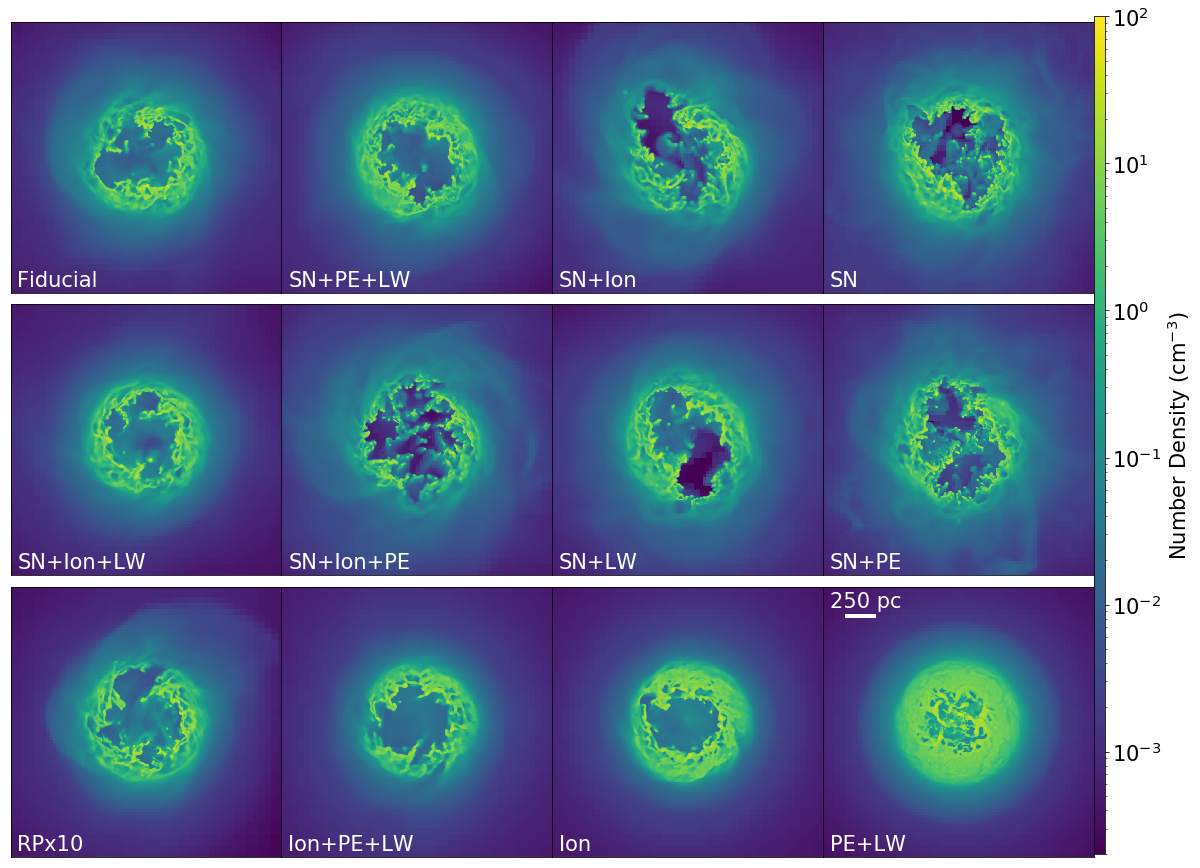
\includegraphics[width=0.95\linewidth]{figures/proj_plot_n_z_125.png}
  \caption{The same panels as Figure~\ref{fig:panel_plot_1}, but face-on.}
  \label{fig:panel_plot_2}
\end{figure*}

In the face-on panels, each galaxy with SNe or ionizing radiation shows a low-density, carved-out circular region at the center, surrounded by a ring of dense gas. The lack of gas in the center of each galaxy is a particular consequence of the large initial burst of star formation present in every case. However, the stellar feedback from SNe and ionization radiation are (alone and together) effective at heating up and driving out cold ISM in the center of galaxy as stars form, which leads to a reduction of the central gas content even outside of this burst phase. Only the Pe+LW run is incapable of removing gas from the center, maintaining a more more uniform and more massive gas disk with localized patches of diffuse gas around newly formed stars. In runs with / without LW and PE (comparing SN+Ion+LW to SN+Ion+PE and SN+LW to SN+PE), LW radiation tends to decrease the presence of dense clumps of gas leading to smaller density contrasts in the inner ISM. As discussed later, this is likely due to the suppression of H$_2$ formation in runs with LW, an important coolant in this low metallicity dwarf galaxy. Many of the clumps seen within the diffuse central region in each simulation are there as projection effects, lying mostly outside the mid-plane of the galaxy.  

In Appendix~\ref{appendix:panels}, we show projection panels at two other points in time for the available simulations to contrast with the panels here, show relatively early in the galaxy's evolution.

\subsection{Global Galaxy Properties}
\label{sec:galaxy properties}

In Figure~\ref{fig:properties} we compare the time evolution of the total \HI~mass, stellar mass, H$_2$ mass fraction, and average ISM metallicity for each of our runs. The \HI~mass in the fiducial simulation declines with time as stars form, radiation ionizes the ISM, and SN feedback drives significant mass loss. Interestingly the H$_2$ fraction increases significantly during this time, but, as shown in Paper~I, this is mostly due to the preferential retention of the cold, dense gas where the H$_2$ resides, rather than the generation of a significant amount of mass of molecular hydrogen. In the bottom right panel we show the evolution of only those metals self-consistently produced by stars formed in the simulation; the initial metal fraction for these species is 10$^{-20}$. In the fiducial run, the mean ISM metallicity remains well below what could be expected for a closed-box, one-zone model (grey, dashed) with the same star formation history. As discussed in Section~\ref{sec:outflows} this is due to the significant outflows generated by feedback in this galaxy. 

\begin{figure*}
  \centering
  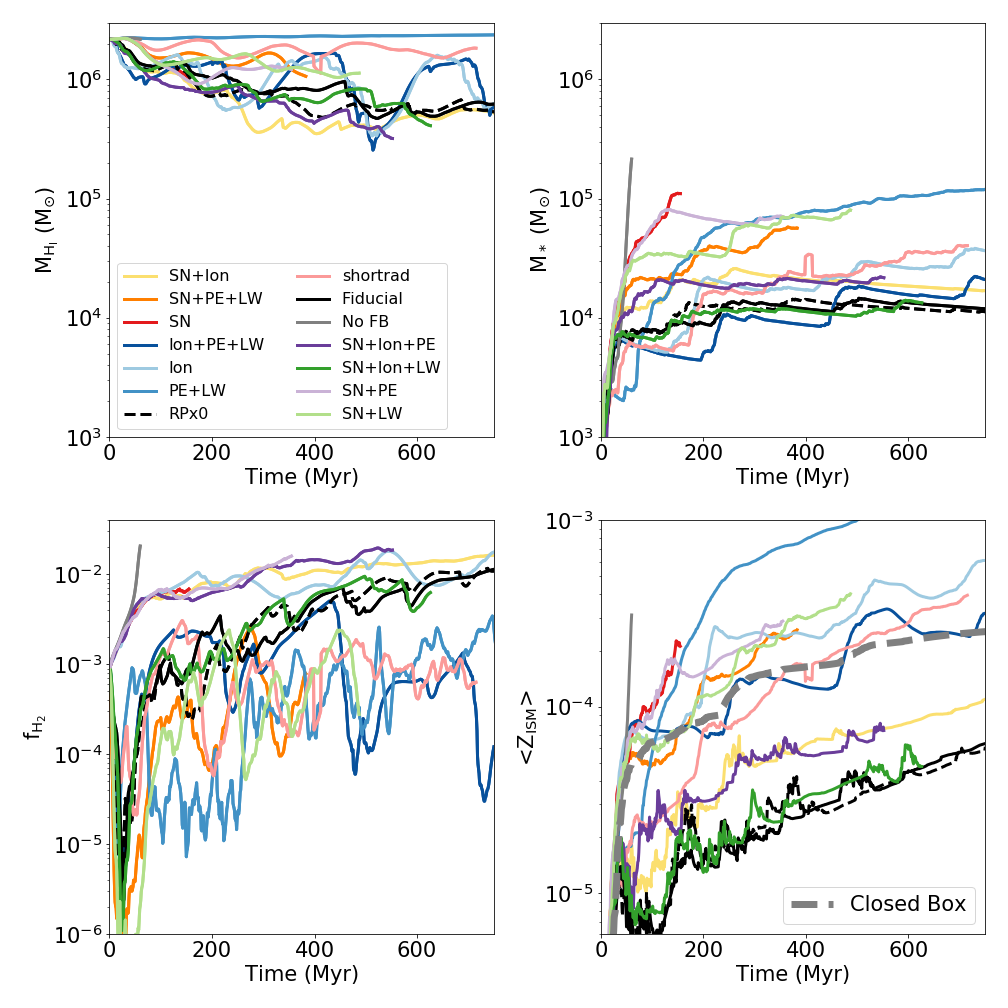
\includegraphics[width=0.98\linewidth]{figures/physics_comparison_masses}
  \caption{The evolution of four global galaxy properties for each of our simulations. Clockwise from top left: \HI mass, stellar mass, H$_2$ fraction, and mean ISM metallicity. $M_{\rm \HI}$ and $M_{*}$ have the same vertical axis limits for comparison of the stellar mass fraction between runs. The $<Z_{\rm ISM}>$ shown here only includes metals self-consistently produced by stars in this simulation (see text). \changed{In the final panel, the grey dashed line shows the corresponding closed-box metallicity evolution for the fiducial simulation.}}
  \label{fig:properties}
\end{figure*}

SN+Ion (along with SN+Ion+PE) generally has the lowest \HI~mass of all of the runs. Compared to the fiducial simulation, this is likely due to the increase in stellar mass and associated increases in feedback strength from both SNe and ionization, which both removes gas in outflows and ionizes \HI~in the ISM. The importance of ionizing radiation in driving the \HI~content is seen clearly comparing to the elevated \HI~masses of all runs without ionizing radiation, especially considering that these runs generally have a higher stellar content. The importance of outflows in regulating the gas content can be seen by comparing Ion+PE+LW (\radstyle) to the fiducial, which shows a similar total stellar mass but greater \HI~content, and the ionization only run (\ionstyle) which has a stellar mass higher than both the fiducial and SN+Ion runs but a comparable \HI~mass to the fiducial run. At the extreme, PE+LW radiation alone clearly is incapable of ionizing or removing any \HI~from this galaxy, in spite of its comparatively high stellar mass. Although the shortrad simulation does contain some ionizing radiation, this localized (within 25~pc) ionizing feedback is clearly insufficient to ionize and remove as much gas as many of the other runs. Looking at the runs with / without PE and LW, including PE from SN to SN+PE (or removing it from the fiducial to SN+Ion+LW) provides little difference in any of these properties. However, adding / removing LW radiation does produce a noticeable effect. 
%We will discuss outflows in more detail in Section~\ref{sec:outflows}.

There appears to be three general groupings in the evolution of the molecular fraction between runs. Runs without LW all exhibit the highest H$_2$ fractions with the smoothest evolution. The remaining runs with LW result in overall lower and more variable H$_2$ fractions. The runs with the lowest H$_2$ content tend to be those that include LW but are missing another form of feedback, leading to increased stellar masses and an increase in the total LW flux in the galaxy. 

%With the exception of Ion+PE+LW (\radstyle) and PW+LW (\pelwstyle) runs, the molecular hydrogen fraction is quite similar throughout the galaxy's evolution. What is most clear from this plot is that stellar LW radiation is indeed important to consider if attempting to model the molecular gas content. The two runs without LW radiation (SN+Ion and ionization-only) show fewer fluctuations in the molecular gas content than the other runs, most obvious during the initial 100~Myr burst where the $H_2$ fractions drop dramatically for those runs with LW radiation. 

Understandably, the differences in stellar mass evolution and gas content in these runs leads to a significant variation in the mean ISM metal fraction. The fiducial run, RPx0, and SN+Ion+LW show the lowest mean ISM metallicities, a factor of $\sim$4 below that of the closed-box model with the same SFH as the fiducial simulation. The remaining simulations show increasing ISM metallicity, driven by a combination of both increased star formation and decreased outflows (greater metal retention). This interplay can be inferred by the fact that the relative differences in $<Z_{\rm ISM}>$ between the various runs and the fiducial simulation are much larger than the same differences in total $M_{*}$. An extreme example of this is comparing PE+LW with SN+PE and SN+LW. All three have somewhat similar total stellar masses by 500~Myr, but significantly different ISM metallicities. We will discuss outflows in more detail in Section~\ref{sec:outflows}.

\subsection{Multi-Phase Gas}
\label{sec:phase diagrams}

%\aje{Its a bit hard to be very precise about this comparison since it's not easy to distinguish feedback effects directly from there just being less / more SF and SNe due to changes in effectiveness of feedback (best example is the RPx0 comparison... I'd expect very little differences, but there are some and its likely not due to lack of RP, but more likely to due sligly different SFR over this time)....might be worth mentioning this as a caution?:}
The properties of the multi-phase ISM for our galaxy simulations is feedback-driven as shown in the temperature-density phase diagrams Figure~\ref{fig:phase_diagram}, and the 1D temperature and density PDFs in Figure~\ref{fig:1D_phase}. Both figures show only gas contained within the disk of each galaxy, and are averaged over a 20~Myr period from 100-120~Myr in each simulation. As indicated by the 2D phase diagrams, the most obvious differences are in the presence / absence of warm/hot ISM ($T > 10^5$~K) driven by SNe that is non-existent in the radiation only runs (bottom right three panels), and the complete absence of diffuse, warm ($T \sim 10^4$~K) gas at $n < 10^{-2}$~cm$^{-3}$ in the run without any feedback. 

Comparing the runs with and without ionization radiation, it is also clear that this feedback component is necessary to maintain a significant amount of gas in the warm, diffuse phases ($10^4~ {\rm K}~ T < 10^5~ {\rm K}$, $n < 1$~cm$^{-3}$). This is most obvious comparing the runs without supernova, but it is also clear that the SN+PE+LW and SN-only runs also have less gas in this regime. Surprisingly, while shortrad does have ionizing radiation feedback, its limited physical extent also reduced the amount of warm, ionized gas compared to simulations with full ionizing feedback. PE and LW radiation seems to have only slight, subtle effects on the gas phases in these figures. However, comparing SN+LW to SN+PE, the latter has slightly more cold, dense gas. The general trends in these diagrams are that including additional feedback sources tends to (overall) broaden the distribution of gas with different densities / temperatures at fixed temperature / density. SNe are necessary to generate hot gas, but are less efficient at sustaining warm/hot, ionized gas. This requires ionizing radiation -- and more than just short-range ionization and heating.

These differences are more distinct in the 1D phase diagrams in Figure~\ref{fig:1D_phase}, giving the full PDFs in the top row and the PDFs normalized to the fiducial simulation in the bottom. Again its clear that runs without SNe lack hot gas, and that this gas is instead piled into the warm phase right around 10$^4$~K. These same runs also have much more cold, dense gas as the lack of SNe makes it challenging to destroy cold gas in the ISM. As suggested previously, LW radiation is important for regulating the presence of cold, dense gas, with SN+PE and SN+Ion+PE havng elevated cold gas compared to their counterparts with LW instead of PE.  
%Comparing the Fiducial simulation with SN+Ion and the radiation only with the ionization only runs, turning off PE+LW has a much less significant effect than turning off ionizing radiation, but it does seem to cha


\begin{figure*}
  \centering
  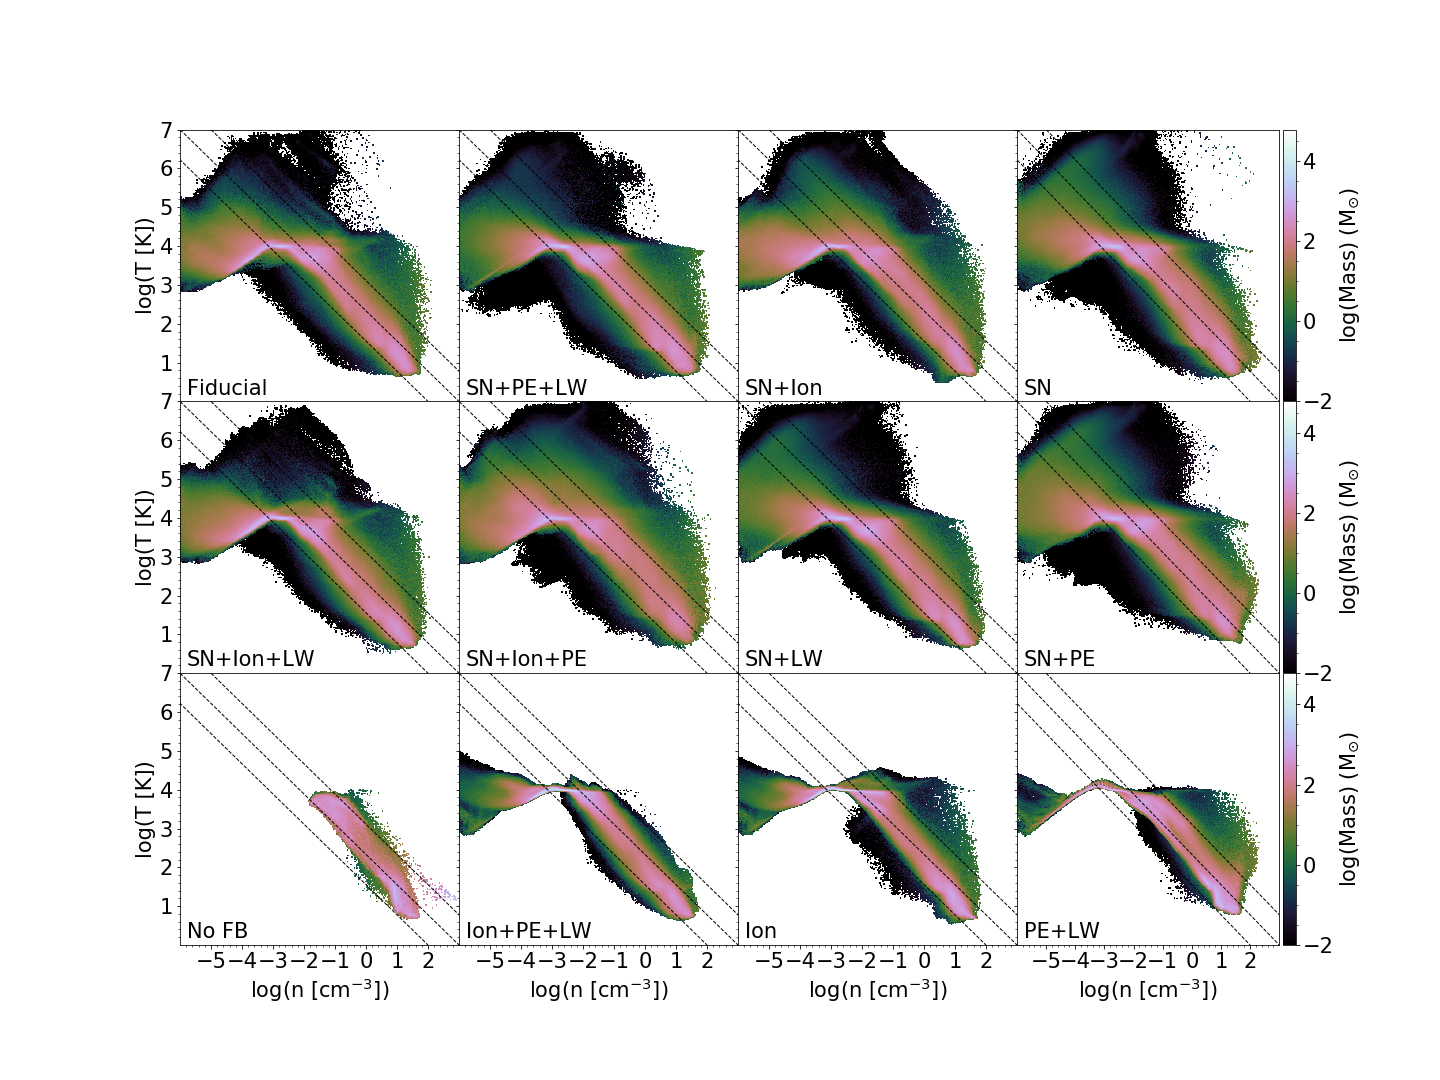
\includegraphics[width=0.95\linewidth]{figures/phase_plot_nT_disk_4x2}
  \caption{The temperature - density phase diagrams for each simulation averaged over the 20~Myr period from 100-120~Myr in each simulation. Lines of constant pressure are given as dashed lines.}
  \label{fig:phase_diagram}
\end{figure*}

\begin{figure*}
  \centering
  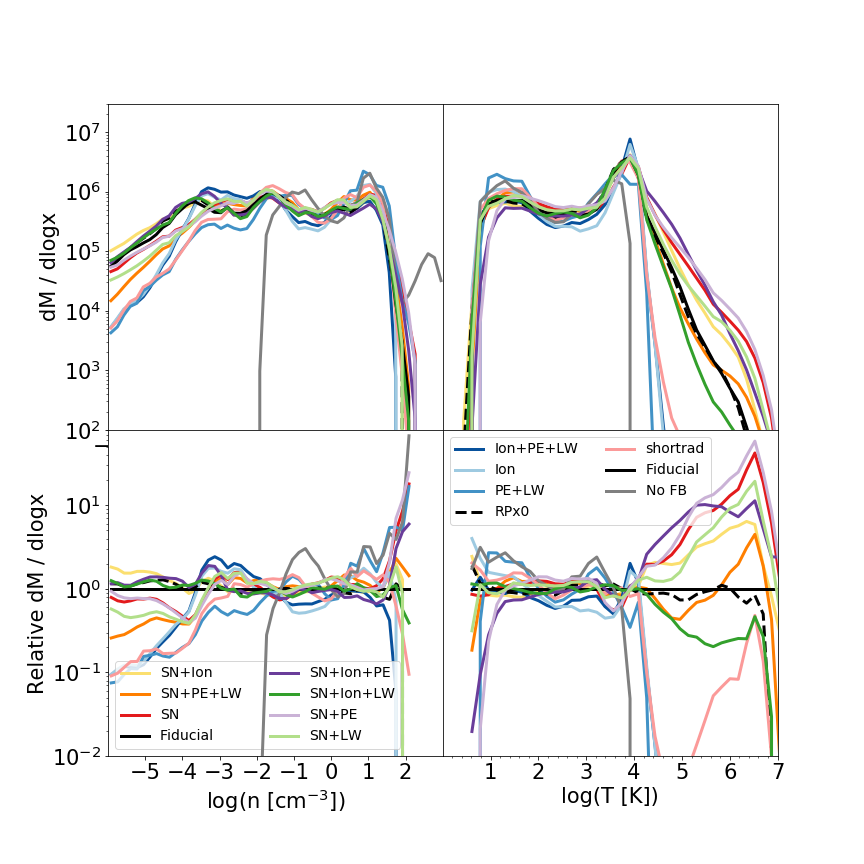
\includegraphics[width=0.95\linewidth]{figures/1D_phase_plot_2panel_nT_phase_disk}
  \caption{The 1D density and temperature PDFs (top) corresponding to Figure~\ref{fig:phase_diagram}, along with each PDF relative to the fiducial simulation (bottom). Line-styles are the same as in Figure~\ref{fig:properties}. \changed{[Changed bin sizes for smoother curves and added legend.]}}
  \label{fig:1D_phase}
\end{figure*}


\subsection{Outflows}
\label{sec:outflows}

Galactic outflows are a natural consequence of stellar feedback, and have been demonstrated to be significant in low mass dwarf galaxies. In Figure~\ref{fig:outflow_evolution} we present the mass outflow rate as measured through an annulus with thickness 0.05~R$_{\rm vir}$ centered at two radii from the galaxy, 0.1~R$_{\rm vir}$ and R$_{\rm vir}$ (again, R$_{\rm vir}$ = 27.2kpc). The total outflow rates in the inner halo are within factors of a few of each other during the first $\sim$200~Myr for all of the simulations except shortrad and PE+LW, which are unable to drive significant outflows. Clearly, some combination of full stellar ionizing radiation and/or supernovae are necessary to drive outflows in low mass dwarf galaxies. 

After this point, the runs differentiate, but generally fluctuate between similar minimum / maximum values. Runs with SN feedback and ionizing radiation tend to maintain a higher, more consistent outflow rate. \changed{The equivalent mass loading factors ($\eta_M \equiv \dot{M}_{\rm out} / \dot{M}_{\rm *}$, and defined in more detail later) for these runs at 0.1~$R_{\rm vir}$ can be between 100 and 400 for all runs including ionizing radiation, and is generally lower (10-50) for those without (and below 1 for PE+LW). This shows that ionizing radiation is important for driving significant outflows, acting on concert with SNe; and in the case of this low mass dwarf galaxy, ionizing radiation alone is capable of driving $\eta \sim$~100 outflows near the disk of the galaxy. It is somewhat surprising that runs without SNe can still reach these large values, but it is the case that 0.1$R_{\rm vir}$ represents a small distance from our galaxy center (2.7~kpc). Only runs with both SNe and ionizing radiation are capable of driving substantial outflows ($\eta > 10$) at the virial radius; PE and LW alone have little impact on the outflows. In agreement with the findings in \citet{Emerick2018a}, how the ionizing radiation feedback is implemented is important, as shown by the low $\eta$ at $R_{\rm vir}$ in the shortrad simulation.}

The efficiency with which stellar feedback drives outflows is often characterized using the mass loading factor, $\eta_M$, metal mass loading factor, $\eta_Z$, and energy loading factor $\eta_E$. We define each of these quantities following \cite{LiBryan2020}: $\eta_M \equiv \dot{M}_{\rm out} / \dot{M}_{\rm *}$, $\eta_Z \equiv \dot{M}_{Z,\rm{out},\rm{SN}} / \dot{M}_{Z,\rm{SN}}$, and $\eta_E \equiv \dot{E}_{\rm out}$. By definition, $\eta_Z$ is always $<$~1 and represents the fraction of SNe-synthesiszed metals that go into outflows. There is some variety in how exactly $\eta_M$ is computed in simulations, even with this definition. $\dot{M}_{\rm out}$ is the instantaneous mass outflow rate, but $\dot{M}_{\rm *}$ is rarely taken to be the instantaneous star formation rate, often time-averaged on anywhere from 1 to 100~Myr. Particularly for galaxies with bursty star formation, as is the case here, exactly how $\dot{M}_{\rm *}$ is averaged can lead to a large variability in $\eta_M$. To smooth over these fluctuations, we use 100~Myr time-averaged $\dot{M}_{\rm *}$ and compute $\eta_M$, $\eta_Z$, and $\eta_E$ every 5~Myr in each simulation for both the hot ($T \geq 3 \times 10^5$~K) and cool ($T < 3\times10^5$~K) phases. \changed{For consistency with the works in \citet{LiBryan2020}, we compute the outflow quantities at a height of 1~kpc above and below the disk of our galaxy.}  We present the average of each of these quantities for each simulation over their entire run-time in Figure~\ref{fig:loading_factors}, as a function of their average star formation rate density.

In general, our simulations show significant amounts of mass and energy driven out via cooler outflows, as the hot loading factors are comparable to or much less than the cooler loading factors. This is qualitatively different from the suite of simulations presented in \cite{LiBryan2020} (see also TIGRESS paper), \changed{[clarified:] where the hot phase carries at least as much mass and energy out as the cold phase.} However, although there is some overlap in $\Sigma_{\rm SFR}$ between our galaxies and a few of the simulations considered in that work, our galaxy has a much lower total mass and gravitational potential. Since the virial temperature of our halo is $1.4 \times 10^4$~K, it is not surprising that both mass and energy can flow out of our galaxy without reaching temperatures above 10$^5$-10$^6$~K. This is further shown by the fact that the two runs with ionization but no SNe have larger mass loading factors driven only by cold gas.

Comparing each run, only the runs with supernovae contain any hot outflows. In general, there is a decreasing trend with $\eta_M$ and star formation rate. However, this trend generally follows the line of constant $\dot{M}_{\rm out}$ for each simulation, suggesting that each galaxy sustains a similar total mass outflow rate, but it is just the efficiency of stellar feedback in driving those outflows that changes by including / excluding different modes of feedback. As shown above, runs with both ionizing radiation and SNe produce the most effiecient outflows -- ejecting more gas per solar mass of star formation than runs without either source of feedback. PE+LW generates the least efficient outflow (near unity $\eta_M$, no metal outflow, and very small $\eta_E$); the SN only run has the highest metal loading, but at a lower mass and energy loading than achieved by also including ionizing radiation. 

It is again insteresting to not the behavior of the shortrad simulation here. It has one of the lowest mass loading factors of runs with SNe, and a metal and energy loading factors more similar to runs without SNe, in spite of the fact that it includes both SNe and ionizing radiation. With reference to the analysis in \citet{Emerick2018a}, it is clear the ionizing radiation is effective at limiting the local star formation in this galaxy, but is not punching diffuse, ionized channels of gas needed for SNe to effectively drive out mass, metals, and energy. This hot gas is trapped, leading to the very low hot loading factors across all three quantities. In runs without ionizing radiation, this is compensated for with extra SNe feedback as the result of additional star formation.

% point for conclusion: self-consistent feedback is key for getting everything right. Not just a matter of getting stellar mass right, but also in concert with outflows and abundances  (AE)

% point for conclusion:, adding in additional non-SN feedback sources changes the mode of outflows from hot-dominated to more cool, (most dramatically with ionization). (AE)

% \aje{Is it worth making a statement about how it might be hard to differentiate between outflow efficiencies if outflows are saturated (at some point, adding more feedback energy won't increase the outflow rate).}

The total $\eta_Z$, which again represents the fraction of SNe-produced metals that outflow relative to the total produced, is fairly uniform for all runs with SNe ($\eta_Z > 0.5$), but significantly lower for those without ($\eta_Z \lesssim 0.1$) and zero for the PE+LW-only run. Comparing to the differences across simulations in $\eta_M$, this raises two important points: 1) while ionizing radiation alone can drive outflows in the inner-halo of this low-mass dwarf galaxy, SNe are necessary to drive metal-enriched outflows, 2) the metal content of SNe-driven outflows in this low-mass dwarf galaxy is less sensitive to additional feedback processes than the total outflows. Cool outflows carry a majority of the metals out of the ISM of our galaxy in each simulation (as is the case for $\eta_M$).

$\eta_E$ shows similar trends except that the differences in energy content between hot and cool outflows are much smaller for some of the runs, and for others $\eta_{E,h}$ exceeds $\eta_{E,c}$ by factors of a few. There appears to be a transition $\Sigma_{\rm SFR}$ around 10$^{-4}$~M$_{\odot}$~kpc$^{-2}$~yr$^{-1}$ above which hot outflows dominate over cold in carrying energy. 

Finally, \citet{LiBryan2020} find a strong correlation between the $\eta_{E,h}$ and $\eta_{Z,h}$ across their examined simulations. We plot the relationship between $\eta_{E}$ and $\eta_{Z}$ and $\eta_{E,h}$ and $\eta_{Z,h}$ in Figure~\ref{fig:loading_relation} (black points) as compared to the simulations presented in \citet{LiBryan2020} (grey points). [changed{[clarified following statement:] We find that there is no strong correlation between the energy loading factor and metal loading factor (left panel) in our simulations; the total energy loading factor is more sensitive to the varying feedback physics than the total metal loading factor. In general, increasing the sources of feedback (particularly SNe and ionization) increases the energy loading factor.} Although our simulations without SNe do not contain any hot outflows, the right panel shows that our simulations exhibit a similar linear relationship between $\eta_{E,h}$ and $\eta_{Z,h}$, but at a slightly higher value ($\sim$1) than in \citet{LiBryan2020} ($\sim$0.4).


\begin{figure*}
  \centering
  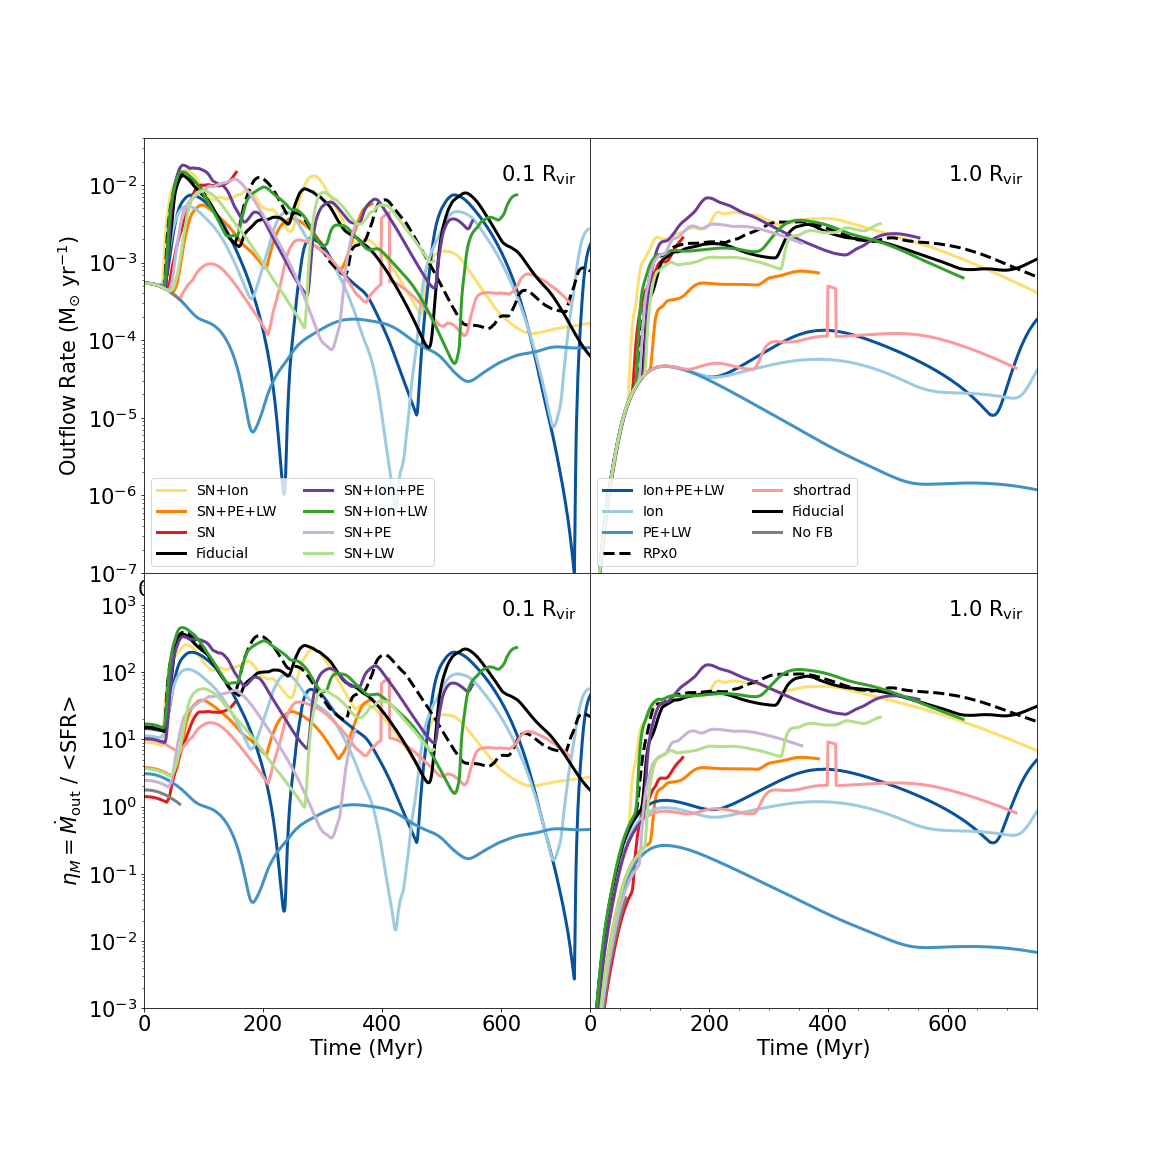
\includegraphics[width=0.95\linewidth]{figures/physics_comparison_outflow_loading}
  \caption{The total mass outflow rate (top) and mass loading factor (bottom) measured at different radii for each of our galaxies. \changed{[added legend]}.}
  \label{fig:outflow_evolution}
\end{figure*}



%\begin{figure*}
%  \centering
%  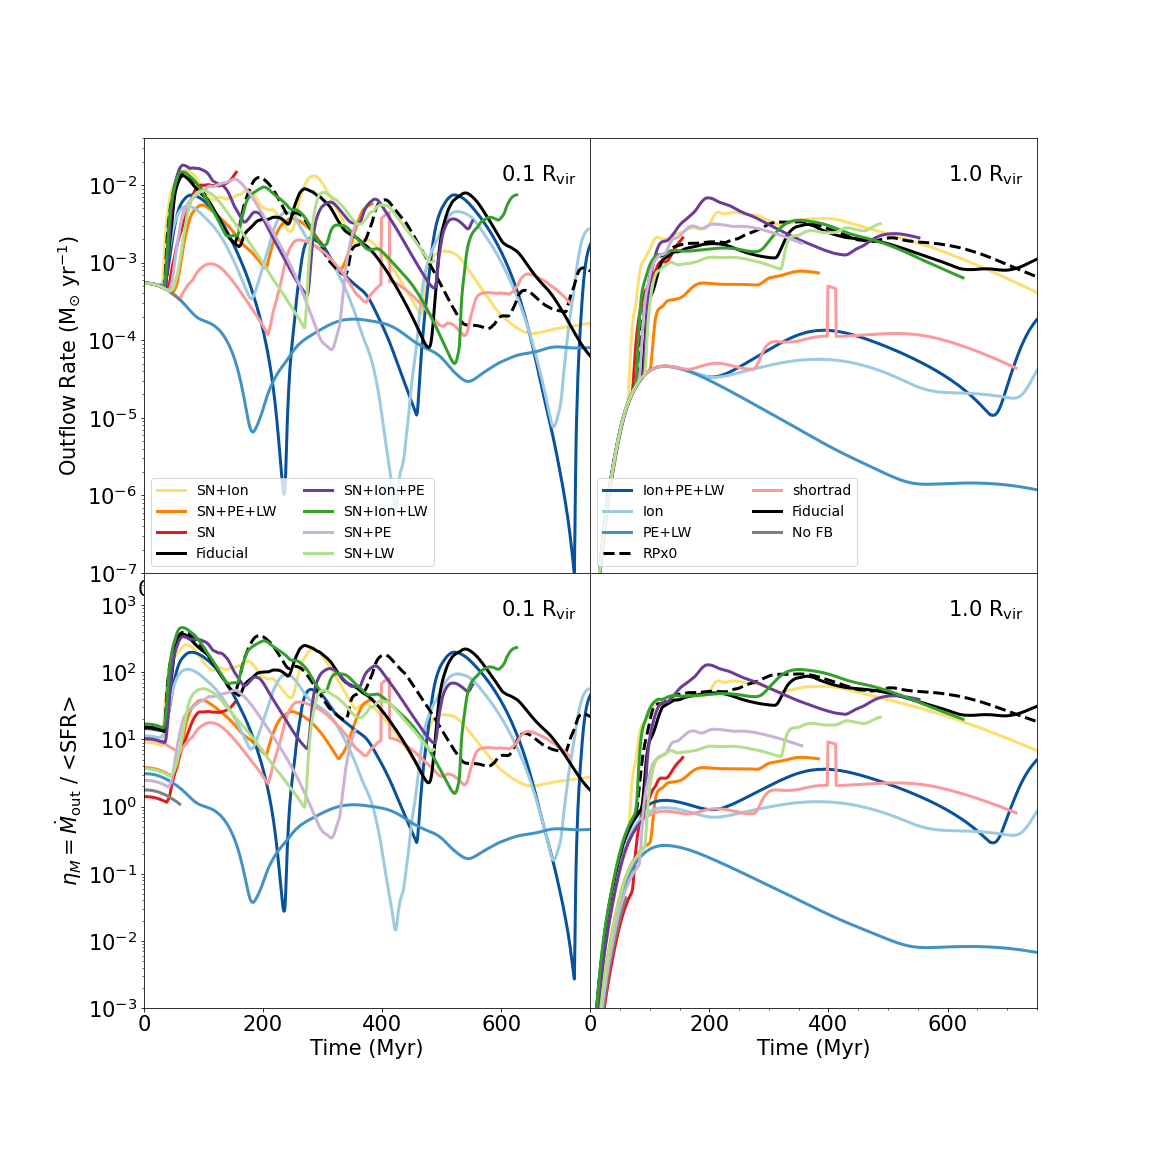
\includegraphics[width=0.95\linewidth]{figures/physics_comparison_outflow_loading}
%  \caption{The mass loading factor measured at different radii for each of our galaxies. For ease of comparison, we use the average SFR over the each entire simulation as the denominator when computing $\eta_M$.}
%  \label{fig:outflow_evolution}
%\end{figure*}

\begin{figure*}
  \centering
  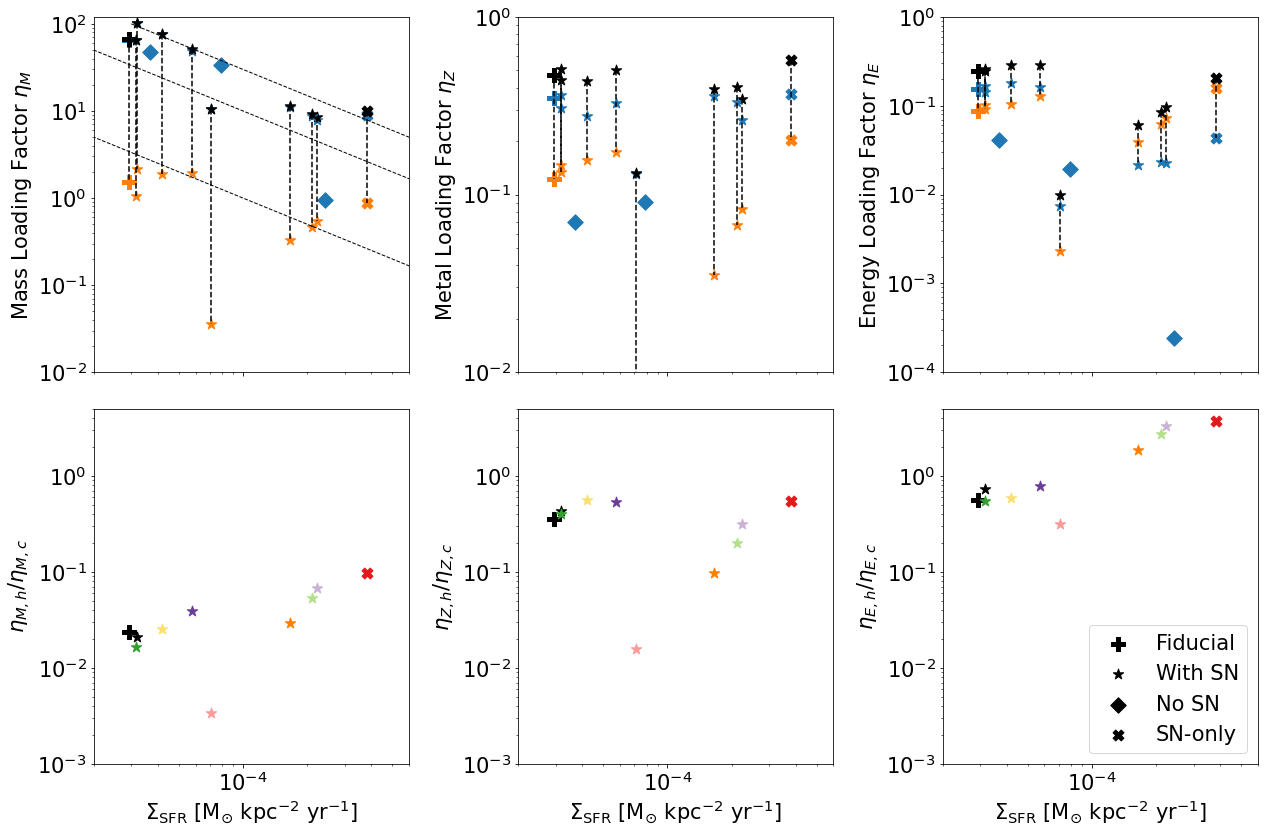
\includegraphics[width=0.95\linewidth]{figures/phys_comparison_mass_metal_hot_cold_SFR}
  \caption{The mass loading factor ($\eta_M$), metal loading factor ($\eta_Z$), and energy loading factor ($\eta_E$) for both hot (orange, $T \geq 3 \times 10^5$~K) and cold (blue, $T < 3 \times 10^5$~K) gas and their ratios for each of our simulations computed at a height of 1~kpc above and below the disk of our galaxy. The totals are shown in the top panel in black, except for the runs without SNe which contain no hot outflows and are left as blue. Each simulation is labelled, but for clarity our fiducial simulation is shown with a plus, simulations with SNe feedback as stars, those without SNe with diamonds, and SN-only with an X. For clarity, the runs without SNe are not separately labelled, but are -- in order of increasing $\Sigma_{\rm SFR}$ -- radiation-only, ionization-only, and PE+LW-only. \aje{I will add in labels by-hand to the SNe runs in final plot. For now, to match up the points with runs, the * runs are (in order of increasing SFR): RPx0, SN+Ion, Shortrad, SN+PE+LW}. The rad-only runs are: radiation, ionization-only, and pe+lw-only}
  \label{fig:loading_factors}
\end{figure*}

\begin{figure*}
  \centering
  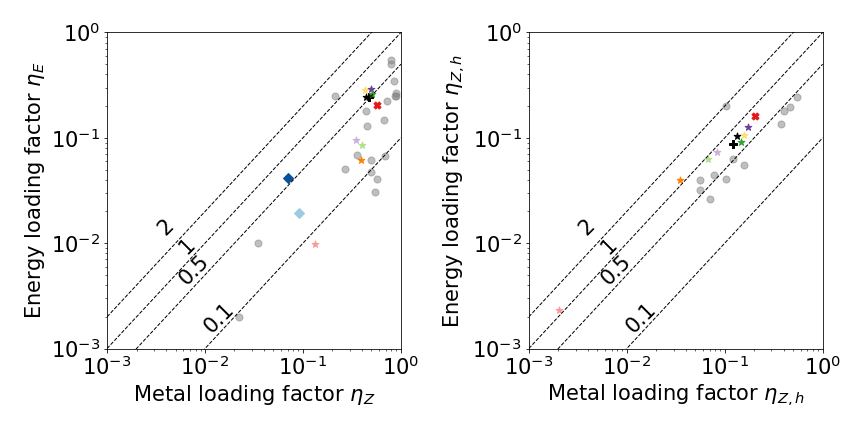
\includegraphics[width=0.95\linewidth]{figures/phys_comparison_E_loading_Z_loading}
  \caption{A comparison of the total and hot energy and metal loading factor relationships for our simulations (black points) as compared to the suite of simulations presented in \citet{LiBryan2020} (grey points), which includes data from \citet{Li2017,KimOstriker2018,Fielding2018,Hu2018,Armillotta2019,Martizzi2016} and \citet{Creasey2015}. Lines of constant $\eta_E / \eta_Z$ are shown.}
  \label{fig:loading_relation}
\end{figure*}

\subsection{Evolution of Individual Metals}
\label{sec:metals}

As explored in \citep{Emerick2018b}, metals released into the ISM in core collapse supernova are ejected from the galaxy through outflows at a higher efficiency than metals from AGB winds. In addition, these same metals showed smaller gas-phase abundance variations -- pointing to more efficient mixing -- than elements from AGB winds. We explore how feedback affects these differences here.

\begin{figure*}
  \centering
  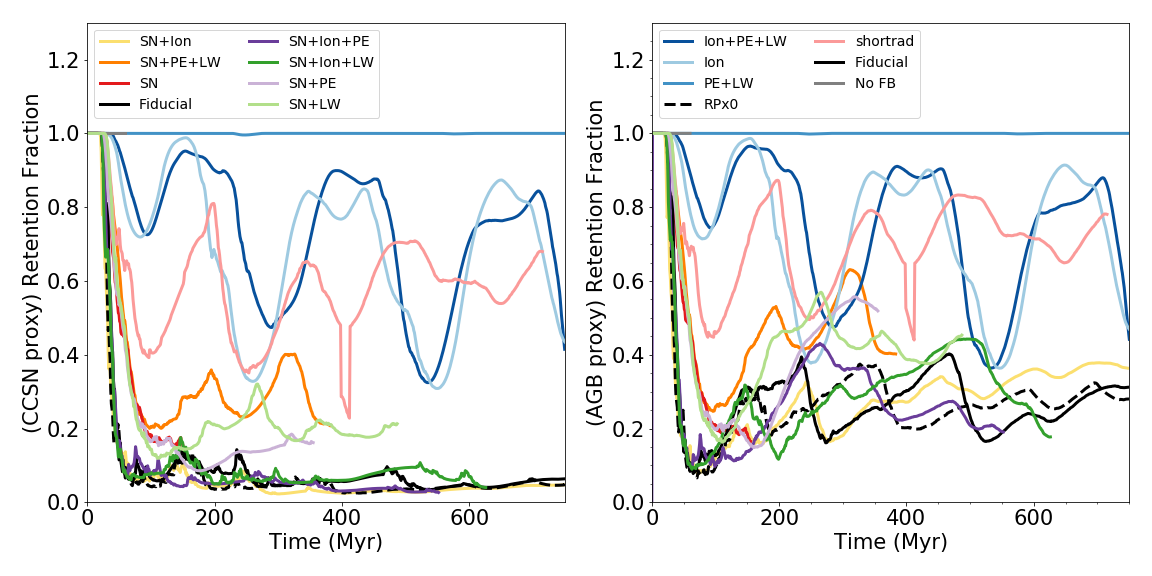
\includegraphics[width=0.95\linewidth]{figures/physics_comparison_retention}
  \caption{The retention fraction of CCSN elements (left, traced by O) and AGB elements (right, traced by Ba) in the disk of each galaxy as a function of time. Line styles are the same as in Figure~\ref{fig:properties}. \changed{[added legend]}.}
  \label{fig:retention}
\end{figure*}

In Figure~\ref{fig:retention} we plot the fraction of metals produced within the disk at each point in time for a CCSN proxy (O, left)\footnote{We note that this quantity does not vary significantly for other SNe-dominated elements, like Mg.} and an AGB enrichment proxy (Ba, right). The fiducial simulation shows a fairly consistent CCSN retention fraction of $\sim$5\% after the first 100~Myr. The AGB retention fraction drops during the first 100~Myr until the first AGB stars begin producing significant Ba; the retention fraction then grows and oscillates with the SFR, but remains between 20\% and 40\%, significantly higher than that for CCSN elements. In general, runs with both SN feedback and ionization show low CCSN element retention. Runs without ionization (SN+PE, SN+LW, SN+PE+LW) retain a much larger fraction of their CCSNe elements (20-40\%), but still have a slightly higher AGB-element retention fractions (40-60\%). Only runs without SNe show similar retention fractions across both CCSNe and AGB elements. The large fluctuations in the shortrad run and Ion and Ion+PE+LW are caused by gas that is removed beyond our formal definition of the disk region, but is not ejected far into the halo and eventually re-accretes onto the galaxy. This is additional confirmation that this difference is due in large part to the difference in energetics between the SN and AGB events, as expected from the analysis in \citet{Emerick2020a}. Retention fractions are similar for different elements if the mode of outflows is dominated by swept-up ISM rather than the direct release of metals from the enrichment source itself (in this case, SNe).  

Although the mass of this galaxy is likely too low to observe the metal content of its circumgalactic medium, where the metals end up beyond the disk of the galaxy may also be an important discriminator between feedback models. We explore this here but for brevity the associated figure is not shown. We find that the fraction of metals in the CGM for CCSN is initially large after the first burst of star formation ($\sim$80-90\%) for all SN runs, but gradually declines to $\sim$20-30\% by the end of the simulation. Since this lost mass is not being re-accreted into the ISM, it is ejected from the halo. Although AGB elements show significantly different disk retention fractions, the CGM fractions are very similar to the CCSN elements. This is possibly because whatever AGB elements do end up in the halo were carried out through the same processes as the CCSN elements, leading to the very similar evolution in the CGM.

%In Figure~\ref{fig:CGM} we plot the gravitationally bound 

\begin{figure*}
  \centering
  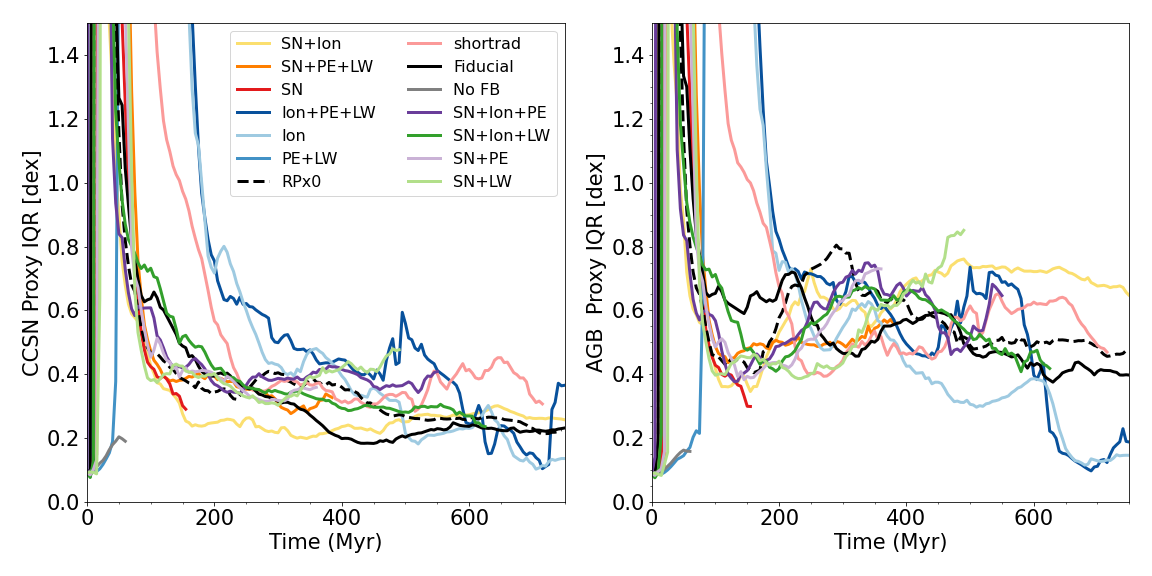
\includegraphics[width=0.95\linewidth]{figures/physics_comparison_IQR}
  \caption{A comparison of the evolution of the inner quartile range (IQR) of the gas-phase abundances of CCSN elements (left, traced by O) and AGB wind elements (right, traced by Ba) in the cold ISM ($T < 10^2$~K). Run Pe+LW (\pelwstyle) remains well above the vertical bounds for the duration of the simulation, and is omitted for clarity (see text).}
  \label{fig:mixing}
\end{figure*}

Finally, we explore the metal mixing differences between these runs and these two elements in Figure~\ref{fig:mixing}. We compare the inner quartile range (IQR) abundance spread of the cold gas for O, the CCSN element proxy, and Ba, the AGB element proxy, for each run. In the fiducial simulation, the CCSN elements show a declining spread throughout the evolution, reaching an IQR of $\sim$0.25 dex by the end of the simulation time. As was seen in the retention fraction, the AGB elements follow the same evolution until the point in time when they are first produced by AGB, at which point the width rises significantly, to around 0.7~dex, and remains well above the CCSN elements until the end of the simulation, though declines to about 0.4~dex. All of the simulations including SN feedback show very similar general trends and final IQR values for O, with the exception of shortrad which takes longer to reach the initial plateu at about 0.4~dex, and stays above the fiducial simulation for the remainder of the time. The comparison here and to the radiation only runs shows the importance that hot-phase mixing has on the evolution of these elements. While the runs with SN hit a roughly consistent IQR after the first $\sim$150~Myr, the runs without SNe take more than twice as long to reach this point. This is in spite of the fact that the radiation-only runs have a higher global SFR with more continual and uniformly distributed enrichment that should allow for more rapid homogenization. However, the radiation only runs do not have SN depositing their elements first in a volume-filling hot phase, which is necessary for rapid mixing over the whole galaxy \citep{Emerick2018b}. However, ionizing radiation does generates some sufficiently warm / hot gas to increasing the mixing timescales over what is present in PE+LW, which is not shown in either panel for clarity. PE+LW exhibits mixing timescales on order or more than the dynamical time of the galaxy ($\sim$1~Gyr); by 300~Myr, this run has an IQR of 10~dex for both elements, declining to 2~dex by 750~Myr in both cases.

Since SN and AGB winds have the same injection energy in the radiation only runs, they exhibit very similar abundance spreads. This suggests that, not only is the mean abundance of individual elements an important discriminator between feedback models, but also the scatter in individual abundances can contain information about the stellar feedback that drives metal mixing in the ISM. Future work correlating gas-phase abundance spreads with ISM properties for a range of feedback models would be useful in making the connection from observed gas-phase abundances to stellar feedback parameters.


\subsection{Stellar abundances}
\label{sec:stellar abundances}

\changed{[removed Type Ia SNe discussion (Fe)]}

The previous discussion focused on the time evolution of the instantaneous gas-phase abundances of the simulated galaxies. But the best observable of galactic chemical evolution in low mass dwarf galaxies is their stellar abundances, which are the convolution of the instantaneous gas-phase abundance distributions and the SFR. To examine the effect of feedback on stellar abundances patterns, we plot the normalized 1D metallicity distribution functions (MDFs) for the abundance ratios [Mg/H]\footnote{The notation [A/B] represents the abundance of element A relative to B, normalized to the solar ratio, in logscale: [A/B]~$\equiv$~log$_{10}$(N$_{\rm A}$/N$_{\rm B}$)~-~log$_{10}$(N$_{\rm A,\odot}$/N$_{\rm B,\odot}$).}, and [Ba/H] in Figure~\ref{fig:MDF1}.\footnote{ While our simulated galaxy is modelled after the $z=0$ properties of the Leo~P dwarf galaxy (see Paper~I), we emphasize that these stellar abundances are likely not representative of the actual abundance patterns in a Leo P like dwarf galaxy ($M_* \sim 10^6 M_{\odot}$) given that we only capture 1~Gyr of evolution. \changed{[added:] It is also for this reason why we do not consider [Fe/H] here or any similar tracer of Type Ia SNe enrichment, as the simulation has not been evolved for a long enough time period for any element to be dominated by this channel (see Figure 2 of \citet{Emerick2018b}).} However, this provides insight into possible abundance variations in lower mass dwarf galaxies who form a majority of their stars over timescales of $\sim$1~Gyr in the early Universe.} These columns represent typical enrichment from ccSNe and s-process enrichment from AGB winds respectively. 

There are three general properties to compare across these MDFs: the location of the peak abundance, the width of the distributions, and the tails towards both higher and lower abundances. The increased peaks in nearly all simulations (compared to the fiducial), with the exception of those in the top panel with both SN feebdack and ionization, is driven by the increase in ISM metals in each case, driven both by lower metal ejection fractions and higher star formation. These distributions are interesting with reference to Figure~\ref{fig:properties}. Simulations with similar $<Z_{\rm ISM}>$ at the point of comparison here, for example, 500 Myr for the shortrad run and $\sim$350 Myr for SN+PE+LW (and also comparing to SN+PE and SN+LW, with slightly higher but still similar $<Z_{\rm ISM}>$) can manifest larger offsets in the peak of their stellar MDFs. This suggests that there is a third mechanism with which stellar feedback regulates stellar abundances. The two obvious, as discussed previously: 1) by modifying the amount of stars that form and thus the number of metals produced and 2) by driving out some fraction of those metals from the ISM, but also  -- more subtle -- 3) by determining how quickly ISM metals can be incorporated into new stars before being ejected. 

The runs with only radiation (bottom panels) also show the higher enrichment compared with the fiducial run, most significantly for PE+LW. Ion and Ion+PE+LW exhibit more similarly peaked MDFs to the remaining SN runs.

\begin{figure}
  \centering
  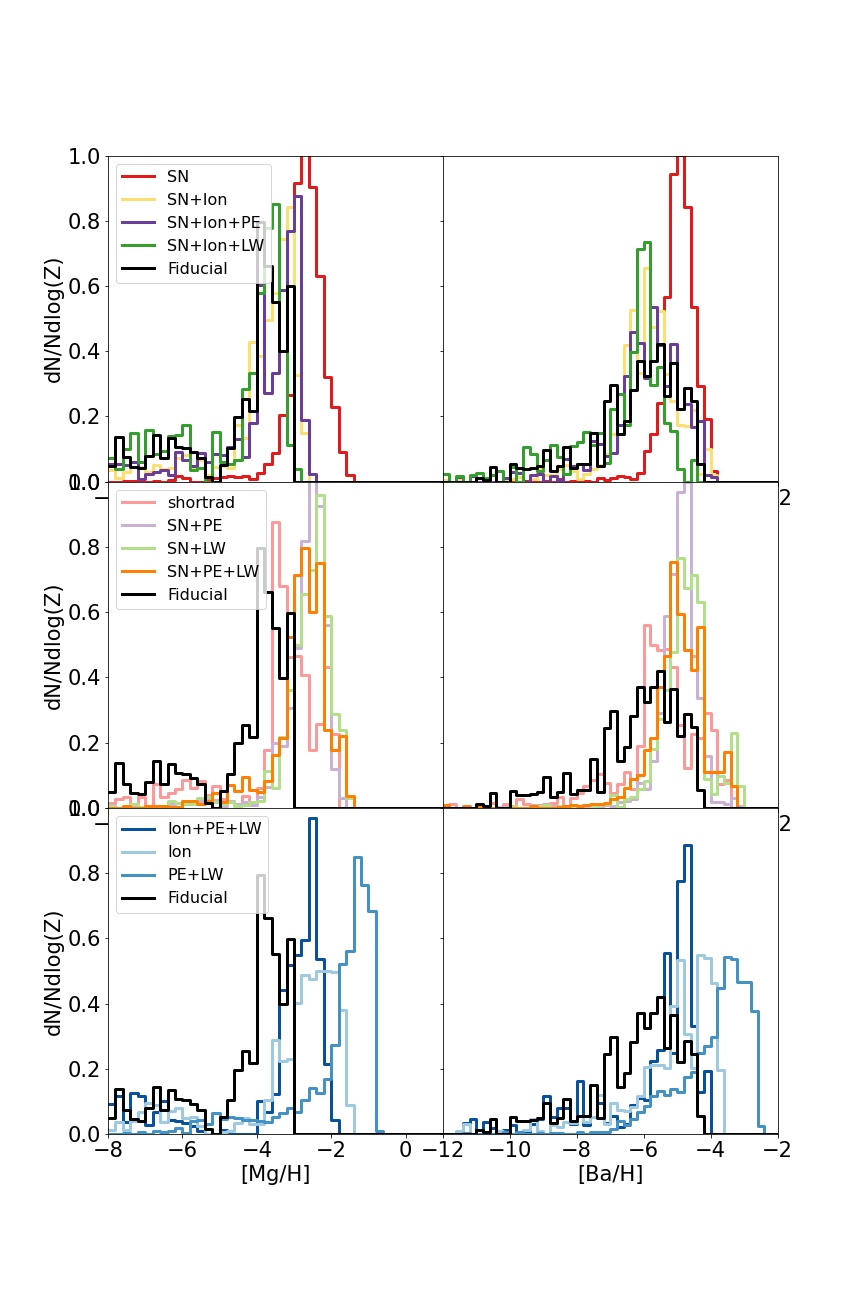
\includegraphics[width=1.1\linewidth]{figures/MgH_BaH_stellar_MDFs}
  \caption{Stellar MDFs for all stars in each simulation at t = 500~Myr (for simulations with final run times less than 500~Myr, we only take those stars that would be alive at 500~Myr). \changed{[removed Fe/H]}}
  \label{fig:MDF1}
\end{figure}

\begin{figure}
  \centering
  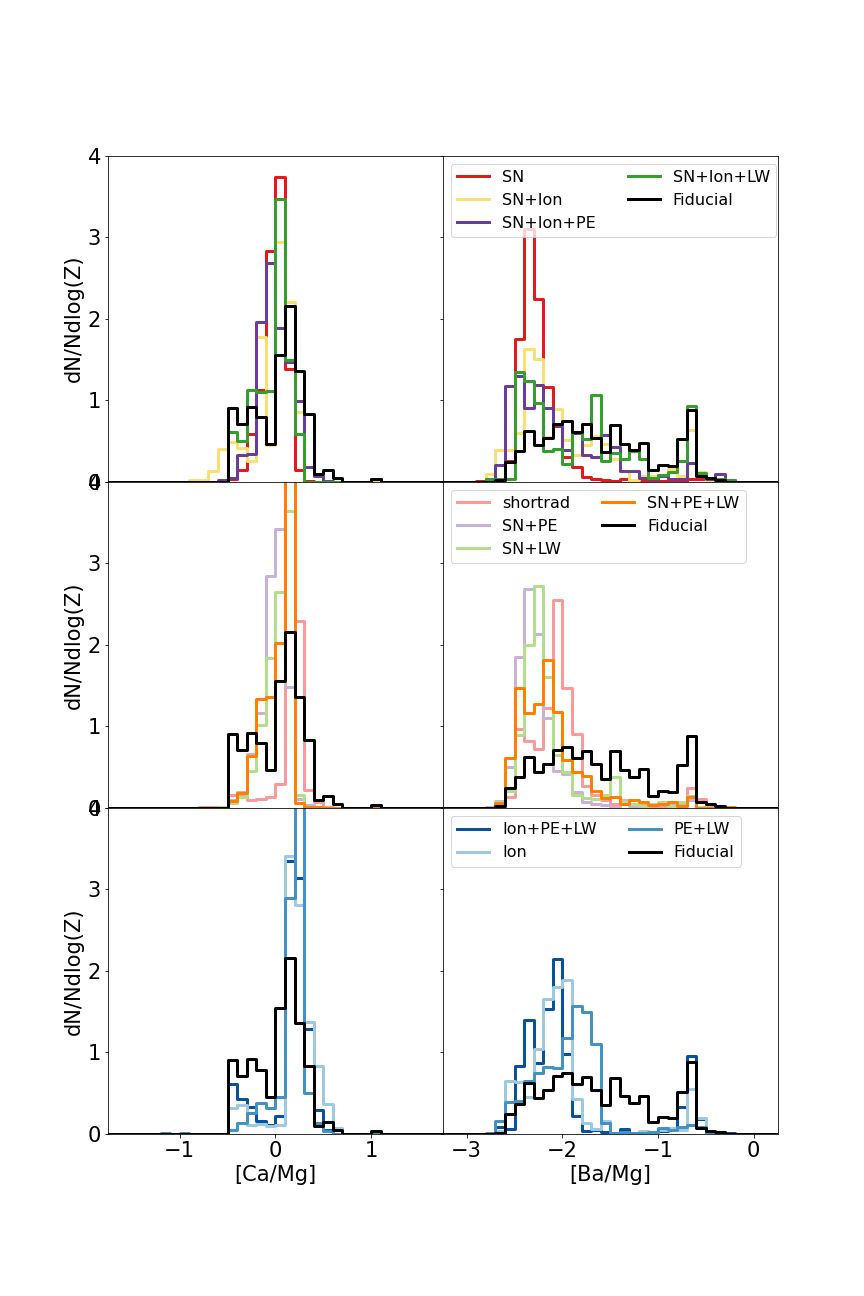
\includegraphics[width=1.1\linewidth]{figures/CaMg_BaMg__stellar_MDFs}
  \caption{The same as Figure~\ref{fig:MDF1}, but for the abundance ratios [Ca/Mg], and [Ba/Mg]. Mg and Ca both trace enrichment from ccSNe, while and Ba traces enrichment from s-process via AGB winds.\changed{[removed Fe/H - still figuring out best linestyles. Using different ratios now]}}
  \label{fig:MDF2}
\end{figure}


While the distribution of stellar abundances in terms of total metal fractions ([X/H]) provides additional insight into the effects of feedback on galactic evolution, this does not necessarily provide any additional constraints that cannot be determined by examining just the total metallicity alone. To examine if individual abundances could provide additional constraints, we plot two abundance ratios in Figure~\ref{fig:MDF2}, [Ca/Mg] and [Ba/Mg]. As shown, the largest differences across all runs lie in the widths of the distributions as compared to the fiducial simulation. In every case, the fiducial simulation produces a broader distribution for each abundance ratio. 

\textbf{(AJE) New:
In [Ca/Mg], the additional star formation and enrichment in each scenario drives the MDF of the distribution closer to the IMF-averaged value of [Ca/Mg] for our yield set ([Ca/Mg] $\sim$ 0.22), homogenizing over some of the mass dependence between these two abundance ratios. This occurs most prominently for the runs with only radiation, and less so for the remaining runs. This is interesteing, because Ca and Mg production varies with supernova type in our yield model, with the most massive (M$_*$ = 25~M$_{\odot}$) producing [Ca/Mg] = -2.96, and least massive (M$_*$ = 8~M$_{\odot}$) having [Ca/Mg] = 0.77 at stellar metal fractions of $Z = 10^{-4}$. The runs with peaks slightly less than the fiducial simulation have peak [Ca/Mg] closer to solar. This suggests a difference in how metals from the first vs. last SNe in a given star formation event are mixed in the ISM and released through outflows. This is an interesting signature of the effects of stellar feedback on stellar abundances beyond differences already shown between metals of different nucleosynthetic sources. However, determining this effect on mass-dependent SNe yields conclusively requires further analysis, in particular the use of tracer particles or separate passive scalar fields in stellar mass bins to conclusively trace the evolution of elements from different SNe.}

In [Ba/Mg], the fiducial simulation and those with both SN and ionizing radiation exhibit broad, nearly flat MDFs across a large range (> 2 dex). The remaining runs all have more narrowly peaked (but still more broad than [Ca/Mg]) distributions around or below [Ba/Mg] of -2. The unifying origin of this difference is in how metals are retained / ejected (Figure~\ref{fig:retention}) across runs. Those with more narrow [Ba/Mg] distributions exhibit greater and more similar retention fractions of both species. It is precisely the relative difference in increased retention fractions between these two species that drives this broadening of these distributions (more retained Mg relative to Ba drives lower [Ba/Mg]). This indicates a second mode for increasing the width of abundance ratio spreads beyond the mixing differences discussed in Section~\ref{sec:metals} and previously in \citet{Emerick2018b}.

This all demonstrates that there are indeed differences in the resulting abundances for models with different stellar feedback, driven by how stellar feedback regulates the SFH of a galaxy relative to the enrichment timescales of different nucleosythnetic processes, and the retention / ejection of different elements in galactic winds.

%A feedback prescription that allows for more rapid, efficient star formation in a galaxy could produce elevated [Mg/Fe] prior to the onset of significant Type Ia contributions. In addition, simulations with less powerful feedback can lead to narrower, more peaked MDFs in multiple abundance ratios. However, these results are not conclusive without additional tests on a range of galaxies with a larger variation in star formation history and galaxy mass. \aje{need a little more here}.


\section{Discussion}

\subsection{Role of Photoelectric Heating}

While photoelectric heating of dust grains is an important source of heating in dense gas of more metal-rich environments like the Milky Way ISM \citep[e.g.][]{BakesTielens1994,Wolfire2003}, its role in low-metallicity dwarf galaxies is unclear. Recently, \cite{Hu2017} found photoelectric heating to be unimportant in a galaxy with stellar mass $\sim$10$^{7}$~M$_{\odot}$ and $Z\sim$0.1~Z$_{\odot}$, in contrast to \cite{Forbes2016} who found it to be a significant source of feedback in their dwarf galaxy of similar mass and metallicity.\footnote{Though see discussion in \cite{Hu2017} which argues the difference was due to a different treatment of metal line cooling in self-shielded gas.} Our results here show more conclusively that photoelectric heating is not a significant source of stellar feedback in the low-metallicity regime of our low mass dwarf galaxy. There is no significant difference between the SN and SN+Pe and the SN+Ion and SN+Ion+PE runs for the properties studied here. Far more important, however, is LW radiation, which does have a significant effect through regulating the H$_2$ content of this galaxy, which is a dominant coolant in this low-metallicity regime. 

\subsection{Radiation Pressure}

The role of radiation pressure in galaxy evolution is also of some debate as to its importance in various regimes \citep[e.g.][]{HQM2011,HQM2012,Agertz2013,Ceverino2014,Sales2015,Rosdahl2015,Kannan2020} (and see also the detailed analysis and discussions in \citet{Krumholz2018} and \citet{Hopkins2019}). In the low-mass dwarf galaxy regime, radiation pressure is sub-dominant to photoheating and ionization, but can still play a significant role in star formation regulation \citep{WiseAbel2012}. We focus here the role of radiation pressure in a low-mass dwarf galaxy in the single-scattering limit, ignoring the potential increase in deposited momentum from resonant re-scattering of UV photons into the IR. In Figure~\ref{fig:RP} we show the cumulative stellar mass, $<Z_{\rm ISM}>$, and mass loading factor $\eta_{M}$ at 0.1$R_{\rm vir}$ for our fiducial simulation and each of the runs varying radiation pressure by a constant multiplicative factor. While there are differences between these runs, the evolution in the first there is no clear trend in any of these results with the radiation pressure factor. RPx0 and RPx2 do not show significant differences from the fiducial simulation. RPx5 and RPx10 do behave differently, but RPx5 forms more stars and RPx10 less than the fiducial. The properties in the reminaing panels do not appear to be dramtically different between these runs.

As this is only a single, isolated low-mass dwarf galaxy we cannot universally say that radiation pressure is subdominant in this regime, but it appears to be unlikely for galaxies much like ours. This is in disagreement with the results from \citet{WiseAbel2012}, which uses the same radiation feedback methods. However, that work studied star formation across a population of dwarf galaxies with different stellar masses and morphologies than the galaxy examined here. This conclusion may also be resolution dependent; higher resolution simulations capable of resolving higher gas densities may see a larger impact from adjusting the effectiveness of radiation pressure.

\begin{figure*}
  \centering
  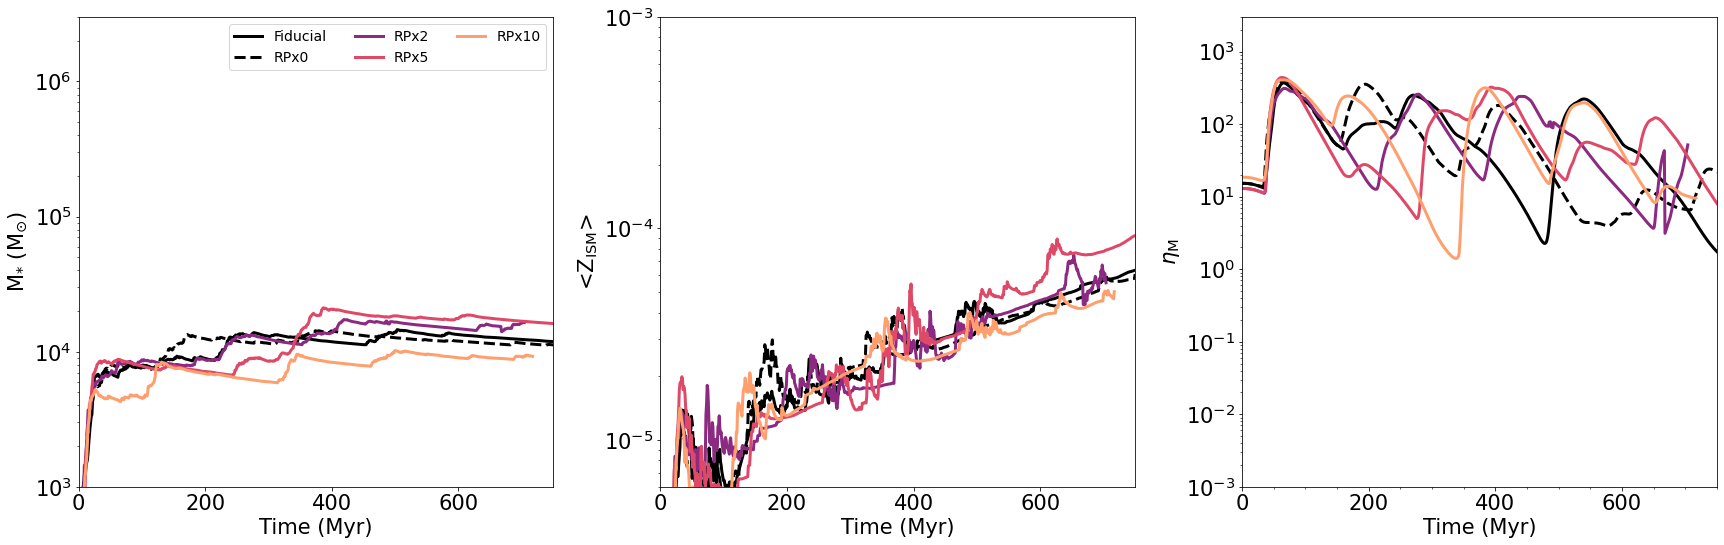
\includegraphics[width=0.95\linewidth]{figures/physics_RP_comparison}
  \caption{A comparison of some of the quantities for the runs varying the effectiveness of radiation pressure.}
  \label{fig:RP}
\end{figure*}

%
% Brainstorm notes: looking at just Fiducial, no ot, no ion, no lw, no pe
%
%   OK. Taking the SN+Ion simulation (solid orange). 
%   Turning ON PE heating leads to a slightly surpressed total SF (so yes PE heating seems to have an effect on galaxy evolution, but not DRAMATIC. This has a similar Z to this run and simular total molecular H. Gas mass (HI) is also similar. So global galaxy props don't change toooo much but just surpressed SFR (just slight heating of disk)?
%
%  SN+Ion, turning ON LW (no PE) leads to FAR surpressed SF (2-3), likely due to the significantly surpressed H_2 fraction in the galaxy (early on especially but also lasting for a while). This leads to a lower ISM metallicity due partly to outflows?
%
%  Ok. here is where it gets fun. Turning BOTH on leads to a more similar evolution to just PE. Seems like LW+PE might serve to 1) kill off some H_2 which affects SF, but PE keeps disk overall stable against SF keeping SFR down as well? Turning off Ionization makes way more stars than everything.
%
% I think I'm going to have to look at a phase diagram and movie of these... really don't know.
%


\section{Conclusion}

\subsection{Dominant Modes of Stellar Feedback in Low Mass Dwarf Galaxies}

In a set of simulations studying the evolution of a low-mass, isolated dwarf galaxy modelled after the z = 0 properties of the Leo~P dwarf galaxy, we explore the effects that each part of a star-by-star model for multi-channel stellar feedback has on the galaxy's evolution. We test the role that PE heating, LW radiation, ionizing radiation, radiation pressure, and SNe have on this galaxy through 17 different simulations at moderately high (3.6~pc) resolution. We find that each form of feedback are capable of generating some form of self-regulated star formation in our dwarf galaxy. However, the combination of these processes produce qualitatively different star formation rates and galaxy properties. Even in cases where the total stellar mass formed is similar across runs, the different feedback channels can produce significant changes in other galaxy properties. We pay particular attention to their ability to drive metal-enriched outflows, metal-mixing, and stellar abundance patterns for different elements in our galaxy.

Due to the complex interplay of different forms of stellar feedback, it is ill-posed to choose one that is the ``most'' important or effective. However, we can conclude the relative effects on galaxy evolution in models that do or do not include certain feedback processes. We find that SNe and ionizing radiation \textit{together} are the dominant sources of stellar feedback regulating star formation, the multi-phase ISM, and driving outflows in this model of a low-mass dwarf galaxy. These feedback channels act together, with ionizing radiation decreasing the ambient ISM density in which SNe explode and carving channels of diffuse gas needed to vent significant amounts of mass, metals, and SNe in outflows. All of our feedback models generate outflows dominated by cool mass and metal loading, in contrast to the hotter outflows in more massive galaxies; this is less true for energy loading, with more comparable hot / cold loading factors in some runs, and larger hot loading factors in runs with $\Sigma_{\rm SFR} > 10^{-4}$~M$_{\odot}$~kpc$^{-2}$~yr$^{-1}$. In general, including ionizing radiation feedback produces cooler mass and metal outflows while increasing the total mass and metal loading factors (more efficient feeedback). 

We find that the destruction of H$_2$ through LW radiation is an important source of feedback in our low-metallicity dwarf galaxy. In this regime, H$_2$ is a dominant coolant and the dominant source of dust formation. This feedback source produces a far greater effect on the star formation and outflow properties of our dwarf galaxy than PE heating from FUV radiation, also due to the limited dust content in this low-mass dwarf galaxy. We additionally explore the effects of radiation pressure and find that an order of magnitude boost in the radiation pressure effectiveness in the single-scattering limit is necessary to noticeably affect the evolution of the galaxy, but the trend as a function of this boost factor is not clear. We conclude that radiation pressure is not a signficant source of feedback for this particular galaxy.

In driving metal-enriched outflows, the presence of stellar feedback changes how metals are retained by and mixed within our galaxy. This manifests itself across simulations as a difference in the ISM metal abundances and abundance spreads which have a significant impact on the stellar abundance patterns in this galaxy. This is predominately observable by examining the total abundance of a given element, but also imprints itself upon the abundance ratios in stellar abundance space. As we found in \citet{Emerick2018b}, elements released in SNe vs. AGB winds are ejected at larger rates and mix more efficiently in our fiducial simulation. The difference between the behavior of these two elements decreases in runs with less forms of feedback than our fiducial run, with turning off ionization and SNe having the largest effects (respectively). We find that runs without ionizing radiation (and also without SNe) produced significantly narrower abundance spreads in [Ba/Mg] (proxies of AGB and core collapse SNe elements, resepctively) than our fiducial simulation. In addition, each simulation shows differences in stellar [Ca/Mg] -- both released in SNe, but with a ratio that is strongly dependent on stellar mass.

In summary, this analysis shows that including a diverse set of stellar feedback modes can drive significantly different star formation, outflow, and chemical abundance properties in low mass dwarf galaxies. While SNe and ionizing radiation are dominant in this regime, LW radiation is also important. Feedback's abilities to drive metal mixing in the ISM and metal enriched outflows, and how it does this differently for elements from distinct sources (e.g. AGB winds vs. SNe) inlfuences the resulting stellar abundance patterns of our dwarf galaxy. This points to the importance of comparing simulations of galaxy to the detailed stellar abundance patterns in observed galaxies as a particularly strong constraint on the underlying physics. This would be best done in high resolution cosmological simulations of galaxy evolution, capable of capturing the details of halo growth and accretion in more realistic environments than the idealized set-up presented here.

%\acknowledgments
\section*{Acknowledgments} AE was supported by \aje{fill in}. \aje{double check:} GLB acknowledges support from NSF grants AST-1615955 and OAC-1835509 and NASA grant NNX15AB20G. M-MML was partly supported by NSF grant AST18-15461. We gratefully recognize computational resources provided by NSF XSEDE through grant number TGMCA99S024, the NASA High-End Computing Program through the NASA Advanced Supercomputing Division at Ames Research Center, Columbia University, and the Flatiron Institute. This work made significant use of many open source software packages. These are products of collaborative effort by many independent developers from numerous institutions around the world. Their commitment to open science has helped make this work possible. 

%mm many citations from citebay.com.  Don't know what to cite for deepdish, so just put a placeholder in.
\software{\textsc{yt} \citep{yt}, \textsc{Enzo} \citep{Enzo2014}, \textsc{Grackle} \citep{GrackleMethod}, \textsc{Python} \citep{VanRossum1995python}, \textsc{IPython} \citep{perez2007ipython}, \textsc{NumPy} \citep{oliphant2006guide}, \textsc{SciPy} \citep{SciPy}, \textsc{Matplotlib} \citep{hunter2007matplotlib}, \textsc{HDF5} \citep{Fortner1998HDF,Koranne2011}, \textsc{h5py} \citep{h5py}, \textsc{Astropy} \citep{astropy:2013,astropy:2018}, \textsc{Cloudy} \citep{Cloudy2013}, and \textsc{deepdish}}

%\begin{figure*}
%  \centering
%  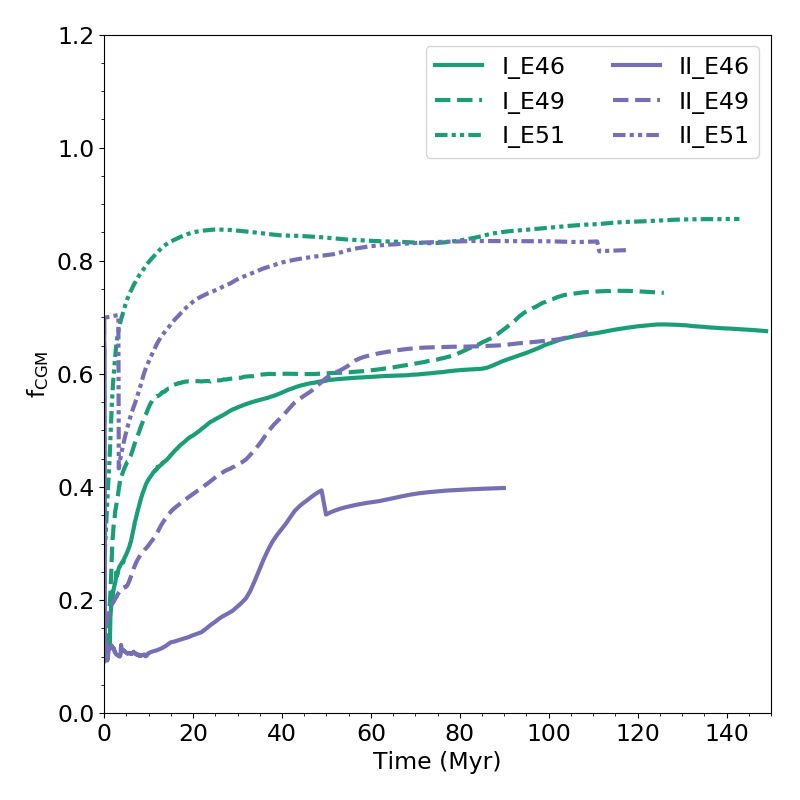
\includegraphics[width=0.45\linewidth]{figures/combined_CGM_average_evolution}
%  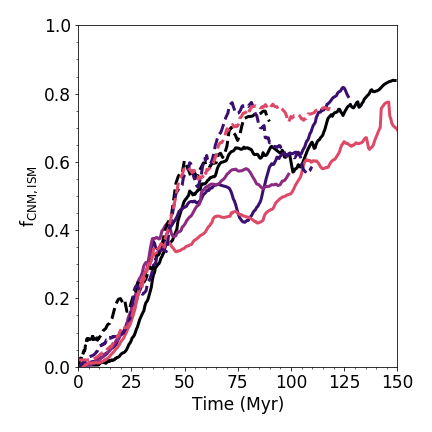
\includegraphics[width=0.45\linewidth]{figures/combined_CNM_average_evolution}\\
%  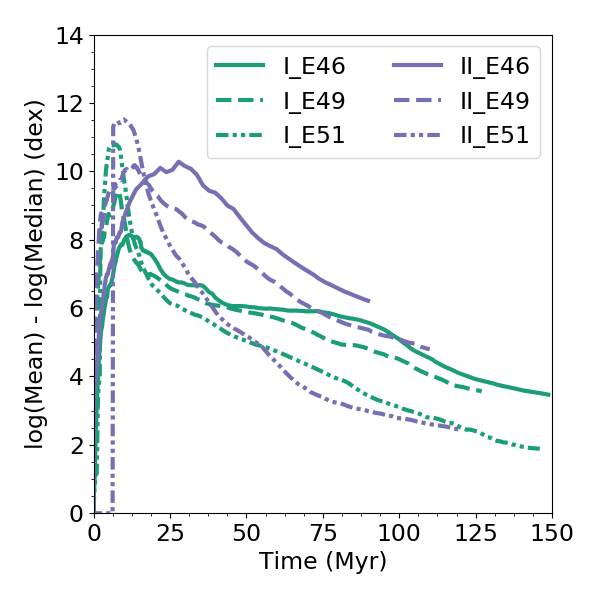
\includegraphics[width=0.45\linewidth]{figures/combined_CNM_average_mean-median}
%   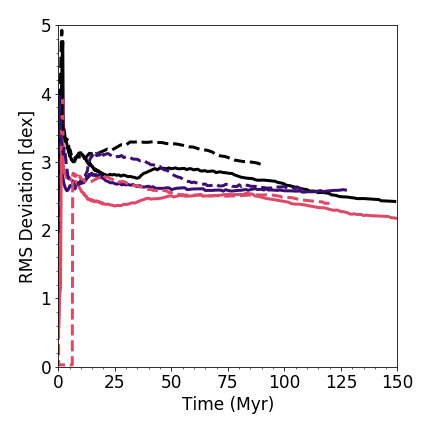
\includegraphics[width=0.45\linewidth]{figures/combined_CNM_average_rms}
%  \caption{The same as Figure~\ref{fig:CGM_CNM} and Figure~\ref{fig:mean-median}, but comparing across both sets of runs with different SFRs. Line color corresponds to a fixed enrichment energy event, while the solid lines correspond to the higher SFR runs discussed throughout this work, and the dashed lines the lower SFR runs. See text for more details.}
%  \label{fig:SFR_comparison_CGM_CNM}
%\end{figure*}


%************* APPENDICES ************************%

%\section*{Acknowledgments}

%\clearpage
\appendix - Liklely DO NOT use this command
\setcounter{section}{0}%
\renewcommand\thesection{\thechapter.\Alph{section}}
\counterwithin{figure}{section}

\section{Morphological Properties}

In Section~\ref{sec:morphology}, we discuss the morphology of our galaxy early in its evolution (125~Myr), just after the initial star formation burst for each simulation and at a time reached by each simulation. We explore here the gas morphology at later, more quiescent times, which are not reached by all simulations.

In Figure~\ref{fig:panel_plot_3} and Figure~\ref{fig:panel_plot_4} we show face-on projections of gas number density at 350~Myr for each simulation. In the edge-on panels, the same general trends seen in Section~\ref{sec:morphology} across runs can be seen here. The largest difference in each panel is the decrease in each case of the amount and morphology of gas beyond the disk of the galaxy. During this period of low SFR for all but the shortrad simulation, the extraplanar gas around the disk is more uniform and less extended than during times of higher SFR. 

This is visible as well in the edge-on panels, which still exhibit the similar lower-density cores and higher-density rings as appeared at t=125~Myr. The key difference is that the lower-density, inner regions have a higher typical density than when the galaxy was actively star forming. In addition, at 350~Myr, the outer rings in each galaxy tends to be clumpier and less continuous, broken up by star formation and feedback over the preceding 250~Myr. PE+LW shows the least variability between these two times, and also has the most uniform SFR of all the simulations. 


\begin{figure*}
  \centering
  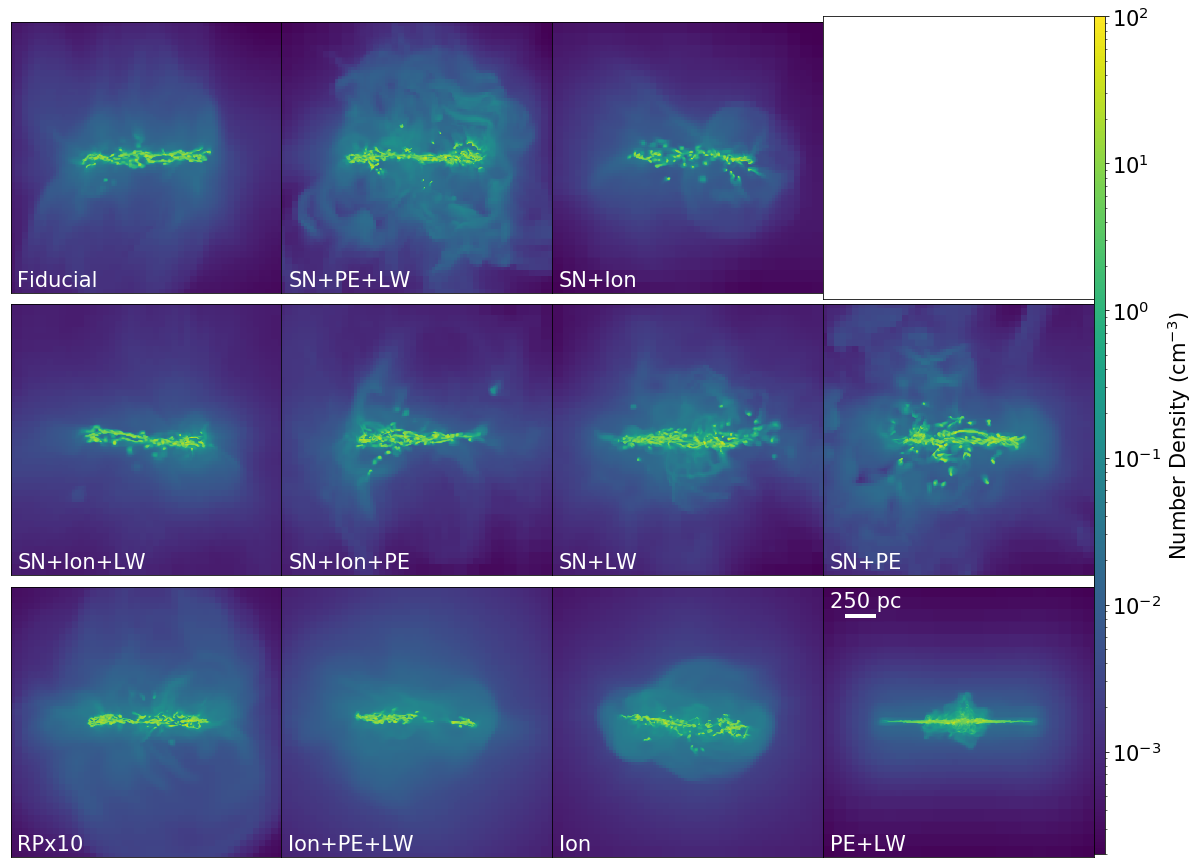
\includegraphics[width=0.95\linewidth]{figures/proj_plot_n_x_350.png}
  \caption{Edge-on projections of gas number density for each of our runs at time $t=350$~Myr for all but the SN-only simulation.}
  \label{fig:panel_plot_3}
\end{figure*}

\begin{figure*}
  \centering
  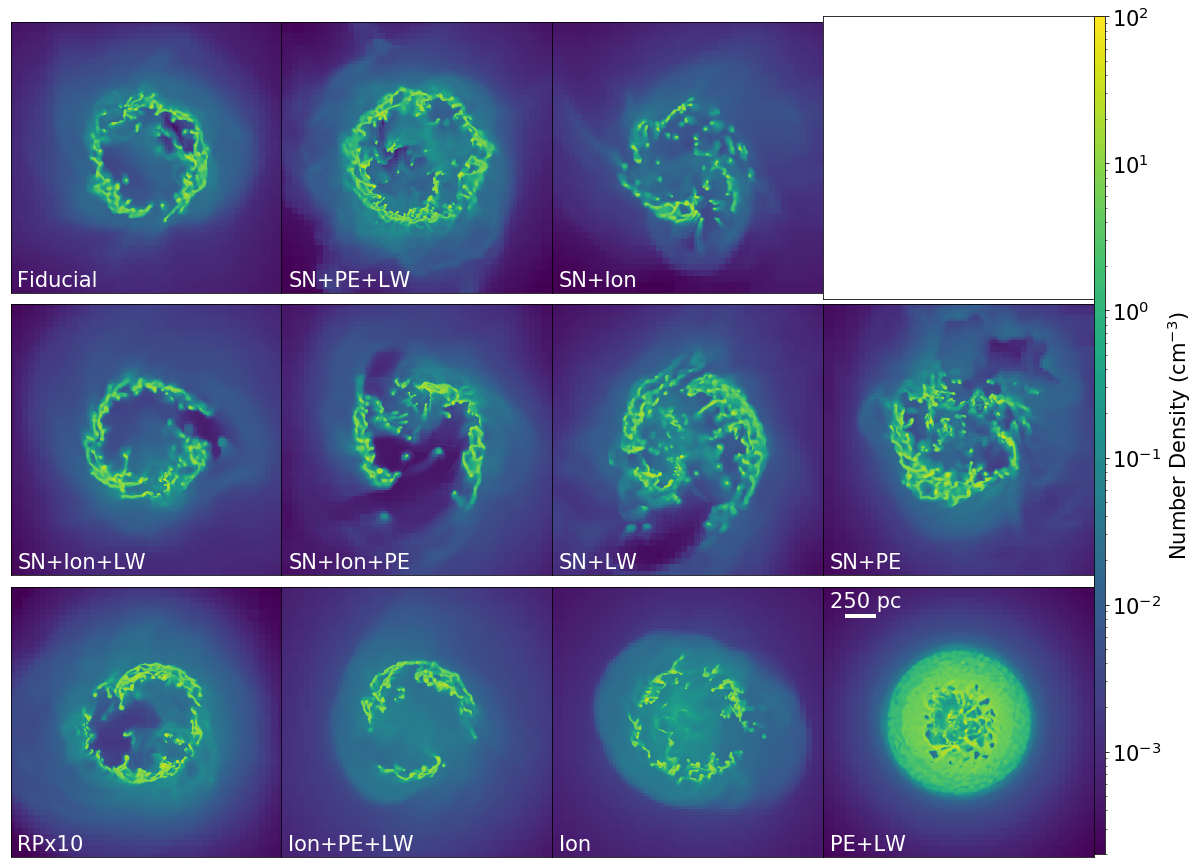
\includegraphics[width=0.95\linewidth]{figures/proj_plot_n_z_350.png}
  \caption{Same as Figure~\ref{fig:panel_plot_3}, but face-on.}
  \label{fig:panel_plot_4}
\end{figure*}
%
%
% Place appendix here%


\bibliographystyle{yahapj}
\bibliography{refs}

\end{document}
